\documentclass[man,12pt,floatsintext,donotrepeattitle]{apa7}

\usepackage[american]{babel}
\usepackage{csquotes}
\usepackage{amsmath,amssymb}
\usepackage{amsthm}
\usepackage{booktabs}
\usepackage{graphicx}
\usepackage{xcolor}
\usepackage{subcaption}
\usepackage[most]{tcolorbox}
\usetikzlibrary{positioning, arrows.meta, fit, calc, decorations.pathreplacing}
\usepackage{needspace}
\usepackage[style=apa,backend=biber]{biblatex}
\addbibresource{refs.bib}
\usepackage{nameref}
\hypersetup{
  hidelinks,
  pdftitle={Rule-Rewriting Cellular Automata and the Edge of Chaos},
  pdfauthor={Joseph Corneli},
  pdfsubject={Permutation-propagators in cellular automata},
  pdfkeywords={cellular automata, rule evolution, Langton's lambda,
    self-modifying systems, edge of chaos, artificial life, permutation
    operators, exhaustive classification, domain walls}
}

\newcommand{\sig}{\sigma}
\newcommand{\bit}[1]{\mathrm{bit}[#1]}
% Sections are unnumbered in apa7 `man' mode, so \ref{sec:..} is empty;
% cross-reference sections by name instead.
\newcommand{\secref}[1]{\emph{\nameref{#1}}}
\newif\ifpaperboxfold
\tcbset{%
  fold/.code={%
    \paperboxfoldtrue
    \pgfkeysalso{top=0pt,bottom=0pt,boxsep=0pt}},
  unfold/.code={\paperboxfoldfalse}}
\newcommand{\foldmark}{%
  \ifpaperboxfold\space{\normalfont\scriptsize[folded]}\fi}

\newtcolorbox[auto counter]{workedexampleframe}[2][]{%
  enhanced,
  breakable,
  colback=green!6,
  colframe=green!45!black,
  boxrule=0.7pt,
  arc=1.5mm,
  left=2.5mm,
  right=2.5mm,
  top=1.5mm,
  bottom=1.5mm,
  fonttitle=\bfseries,
  title={Worked example~\thetcbcounter: #2\foldmark},
  #1}
\NewDocumentEnvironment{workedexample}{O{} m +b}{%
  \paperboxfoldfalse
  \begin{workedexampleframe}[#1]{#2}%
    \ifpaperboxfold\else#3\fi
  \end{workedexampleframe}}{}

% --- typed boxes for compression -------------------------------------------
% Each typed box accepts `fold` in its option list. Folding preserves its
% counter, title, label, and cross-references while suppressing only the body.
\newtcolorbox[auto counter]{theoremframe}[1][]{%
  enhanced, breakable, colback=blue!5, colframe=blue!55!black,
  boxrule=0.7pt, arc=1.5mm, left=2.5mm, right=2.5mm,
  top=1.5mm, bottom=1.5mm, fonttitle=\bfseries,
  title={Theorem~\thetcbcounter\foldmark}, #1}
\NewDocumentEnvironment{theorem}{O{} +b}{%
  \paperboxfoldfalse
  \begin{theoremframe}[#1]%
    \ifpaperboxfold\else#2\fi
  \end{theoremframe}}{}

\newtcolorbox[auto counter]{definitionframe}[2][]{%
  enhanced, breakable, colback=violet!6, colframe=violet!55!black,
  boxrule=0.7pt, arc=1.5mm, left=2.5mm, right=2.5mm,
  top=1.5mm, bottom=1.5mm, fonttitle=\bfseries,
  title={Definition~\thetcbcounter: #2\foldmark}, #1}
\NewDocumentEnvironment{definition}{O{} m +b}{%
  \paperboxfoldfalse
  \begin{definitionframe}[#1]{#2}%
    \ifpaperboxfold\else#3\fi
  \end{definitionframe}}{}

% Corollaries auto-boxed like theorems (blue). Empirical findings are amber:
% observed (not proved) claims live here, the validated home for rewritten results.
\newtcolorbox[auto counter]{corollaryframe}[1][]{%
  enhanced, breakable, colback=blue!5, colframe=blue!55!black,
  boxrule=0.7pt, arc=1.5mm, left=2.5mm, right=2.5mm,
  top=1.5mm, bottom=1.5mm, fonttitle=\bfseries,
  title={Corollary~\thetcbcounter\foldmark}, #1}
\NewDocumentEnvironment{corollary}{O{} +b}{%
  \paperboxfoldfalse
  \begin{corollaryframe}[#1]%
    \ifpaperboxfold\else#2\fi
  \end{corollaryframe}}{}

\newtcolorbox[auto counter]{propositionframe}[2][]{%
  enhanced, breakable, colback=blue!5, colframe=blue!55!black,
  boxrule=0.7pt, arc=1.5mm, left=2.5mm, right=2.5mm,
  top=1.5mm, bottom=1.5mm, fonttitle=\bfseries,
  title={Proposition~\thetcbcounter: #2\foldmark}, #1}
\NewDocumentEnvironment{proposition}{O{} m +b}{%
  \paperboxfoldfalse
  \begin{propositionframe}[#1]{#2}%
    \ifpaperboxfold\else#3\fi
  \end{propositionframe}}{}

\newtcolorbox[auto counter]{empiricalfindingframe}[2][]{%
  enhanced, breakable, colback=orange!7, colframe=orange!65!black,
  boxrule=0.7pt, arc=1.5mm, left=2.5mm, right=2.5mm, top=1.5mm, bottom=1.5mm,
  fonttitle=\bfseries,
  title={Empirical finding~\thetcbcounter: #2\foldmark}, #1}
\NewDocumentEnvironment{empiricalfinding}{O{} m +b}{%
  \paperboxfoldfalse
  \begin{empiricalfindingframe}[#1]{#2}%
    \ifpaperboxfold\else#3\fi
  \end{empiricalfindingframe}}{}

% Empirical findings live canonically in the literate notebook submitted as
% Supplement 1. Keep only stable, compact pointers in the narrative.
\newcommand{\suppfindingref}[1]{Supplement~1, Box~#1}
\newcommand{\suppfinding}[2]{%
  \par\smallskip\noindent\emph{\suppfindingref{#1}: #2.}\par\smallskip}

% Observations (teal): consequences/remarks pulled out of definitions and prose.
\newtcolorbox[auto counter]{observationframe}[2][]{%
  enhanced, breakable, colback=teal!7, colframe=teal!55!black,
  boxrule=0.7pt, arc=1.5mm, left=2.5mm, right=2.5mm, top=1.5mm, bottom=1.5mm,
  fonttitle=\bfseries, title={Observation~\thetcbcounter: #2\foldmark}, #1}
\NewDocumentEnvironment{observation}{O{} m +b}{%
  \paperboxfoldfalse
  \begin{observationframe}[#1]{#2}%
    \ifpaperboxfold\else#3\fi
  \end{observationframe}}{}

\title{Rule-Rewriting Cellular Automata and the Edge of Chaos}
\shorttitle{Rule-Rewriting Cellular Automata}
\authorsnames{Joseph Corneli}
\authorsaffiliations{{Oxford Brookes University, Oxford OX3 0BP, United Kingdom},
  {Hyperreal Enterprises Ltd, United Kingdom}}
\note{Corresponding author: Joseph Corneli,
  \href{mailto:jcorneli@brookes.ac.uk}{jcorneli@brookes.ac.uk}.}

\abstract{%
We study a two-layer cellular automaton in which each cell carries both a
phenotype state and an eight-bit rule. A permutation $\sig$ of the eight
displayed truth-table positions defines an operator $P_\sig$ on those rules by
$\bit{\sig(p)} := \lnot\,\bit{p}$. The resulting family of $8! = 40{,}320$
permutation-propagators admits exact classification rather than sampling:
$P_\sig$ has a fixed rule exactly when every cycle of $\sig$ is even, an
all-even permutation with $k$ cycles has $2^k$ fixed rules, and every fixed rule
is balanced, with Langton activity $\lambda = 1/2$.

That last result is our point of departure. It places every fixed point of every
operator at exactly the value the classical picture associates with the
transition, and so leaves $\lambda$ powerless to distinguish an operator whose
rule field stays diverse from one that collapses. The dynamics bear this out: a
census across all cycle types separates sustaining from collapsing operators
where $\lambda$ cannot, and a finite-size scan over $L = 30$--$240$ finds a
broad, drifting crossover rather than a sharpening critical point. The classical
search, conducted in parameter space, returns nothing.

We then leave the permutation core while retaining the same two-layer
genotype--phenotype substrate. The objects are now update
\emph{architectures}---temporal schedules, phenotype-reading constructions,
mutation, holding, and conservative transport---rather than individual members
of either the $8!$ or $8^8$ writing families. Flipping one cell and tracking
divergence against an otherwise identical run places one phenotype-reading
construction between elementary rules $90$ and $54$ on a damage-spreading scale
calibrated against rules of undisputed regime. Sustained rule diversity looked
like the order parameter the classical account wants; a conservative control
that holds the rule histogram exactly invariant while varying transport shows
that it is not, reach being nearly flat in diversity and moving by an order of
magnitude with transport. Within the tested architectures, causal reach
separates instead by \emph{coupling}: treating the phenotype-to-genotype edge as
a graded quantity moves reach monotonically across the calibrated scale, while
a mobility-matched control blind to the phenotype remains in the low-reach
band. The exact classification therefore describes the permutation core; the
causal result describes a feedback-coupled extension of it.}
\keywords{cellular automata, rule evolution, Langton's lambda,
self-modifying systems, edge of chaos, artificial life, permutation operators,
exhaustive classification, damage spreading, perturbation analysis}

% Artificial Life asks for the abstract and keywords on the cover page and the
% main text on page 2. In apa7 manuscript mode, suppress the page break that
% normally separates the title page from the abstract; retain the following
% page break before the main text.
\makeatletter
\patchcmd{\maketitle}{\vspace*{4\baselineskip}}{\vspace*{\baselineskip}}%
  {}{\PackageError{draft5}{Could not compact title-page spacing}{}}
\patchcmd{\maketitle}{\newpage}{\vspace{0pt}}%
  {}{\PackageError{draft5}{Could not place abstract on title page}{}}
\makeatother

\begin{document}
\maketitle

\section{Two Readings of the Edge of Chaos}
\label{sec:intro}

In 2015, working on a different problem, we built a cellular automaton
whose cells carried rules rather than states
\parencite{corneli2015search}.  A programming error connected with one
example generated spacetime diagrams reminiscent of the edge of chaos
behaviour observed in classical CAs.  The question of how that example
recovered the distinctive visual behaviour remained open.

Recent computational experiments have located that accidentally discovered
operator within a larger landscape. A permutation $\sig$ of the eight
truth-table positions of an elementary rule defines an operator $P_\sig$ that
rewrites a rule by negating the bits $\sig$ names; there are $8! = 40{,}320$
such operators, and they admit exact classification rather than sampling. They
form the bijective core of the $8^8$ possible writings. The original example
recreated in Figure~\ref{fig:fig2pair} is a non-bijective writing outside that
core. We therefore separate two objects that share a substrate but not a scope:
the finite permutation core studied in Part~I, and the wider class of
state-dependent update architectures studied in Part~II.

The classical literature offers two readings of ``the edge of chaos'', and they
are different kinds of object. The first is a location in \emph{parameter
space},
aligned with an order parameter which can be tuned so that the dynamics sit
between order and disorder \parencite{langton1990computation}. Our
classification lands on it from an unexpected direction---every fixed rule of
every operator in the family is balanced, with Langton activity
$\lambda = 1/2$, exactly the value the classical picture associates with the
transition. Yet searching the Meta Cellular Automaton (MetaCA) for a critical
transition does not produce one (\suppfindingref{7}). The
algebra places the fixed points precisely at the classical critical value; the
dynamics show a broad, drifting crossover and no critical point of that sort at
all.

The second reading is not a boundary one tunes toward but a region one measures
the system into. It is dynamical: an
ordered system absorbs a perturbation, a chaotic one lets it fill the light
cone, and the interesting regime lies between. That reading requires no
parameter sweep and no choice of where to draw a region---it requires only a
perturbation and a clock. Flipping a single cell and tracking the divergence
against an otherwise identical run, on a scale calibrated against elementary
rules whose regime is not in dispute, places the phenotype-reading construction
of \secref{sec:braiding} between rules $90$ and $54$, below rule $110$ and far
below the chaotic rule $30$, while frozen rules return exactly zero
(\secref{sec:causal}). The live phenotype-to-genotype coupling is what puts it
there: cutting that single edge, with seed, tape and construction otherwise
identical, roughly halves how far a perturbation reaches.

Pursued far enough, the second reading also tests and rejects a tempting
substitute for the classical order parameter. Across seven mechanisms, causal
reach initially appears to rise and then fall with sustained genotype
diversity, but the descending observations obtain high diversity only through
mutation or by holding rules still. A conservative eighth construction
prescribes the genotype measure and transports it by local bijective exchanges.
It sustains causal amplification across the full $32$--$256$ rule range:
exchange rate, not diversity alone, controls reach
(\secref{sec:diversity-axis}).

Placing the tested architectures on the calibrated scale then identifies a
candidate control within the extension. The
constructions separate by \emph{coupling}: where the genotype update never reads
the phenotype---the bare operators, braids, niches, refuges, mutation, and blend
strength across its whole range---nothing clears the bottom of the complex band,
while everything that reads it lands inside (\suppfindingref{11}). The coupling
is moreover a dial rather than a switch. Tuning the gain of that loop carries reach smoothly from the frozen
identity past rules $90$, $110$ and $54$, with a locatable crossing; an ungated
control matched in mobility, differing only in that its rewriting is blind to
the phenotype, never leaves the ordered band. Within these constructions the
classical picture is therefore recovered in a coordinate it does not usually
use: not a truth-table parameter, but the gain of the loop from the phenotype
back to the genotype.

This is the paper's edge-of-chaos claim, and its scope is the feedback-coupled
extension, not the $8!$ family as a whole. It is measured rather than assumed:
in the tested construction, adding the phenotype-to-genotype edge carries
causal reach into the calibrated complex band and cutting it carries reach back.

Supplement~2 reports a separate exploratory analysis of
coexisting spatial domains and documents a boundary-transport statistic
withdrawn after a circularity check. Neither is used to support either
edge-of-chaos claim here.

Part~I classifies the permutation-propagators, surveys their spatial dynamics,
and tests the parameter-space reading of the edge of chaos. Part~II explicitly
drops the restriction to a single permutation-propagator and studies causal
reach in update architectures built on the same genotype--phenotype substrate.
The exact results hold for the entire $8!$ core. The causal measurement covers
one principal construction at one lattice width over six seeds, and no
comparable causal census of either the $8!$ or $8^8$ family is attempted here.

\begin{figure}[H]
\centering
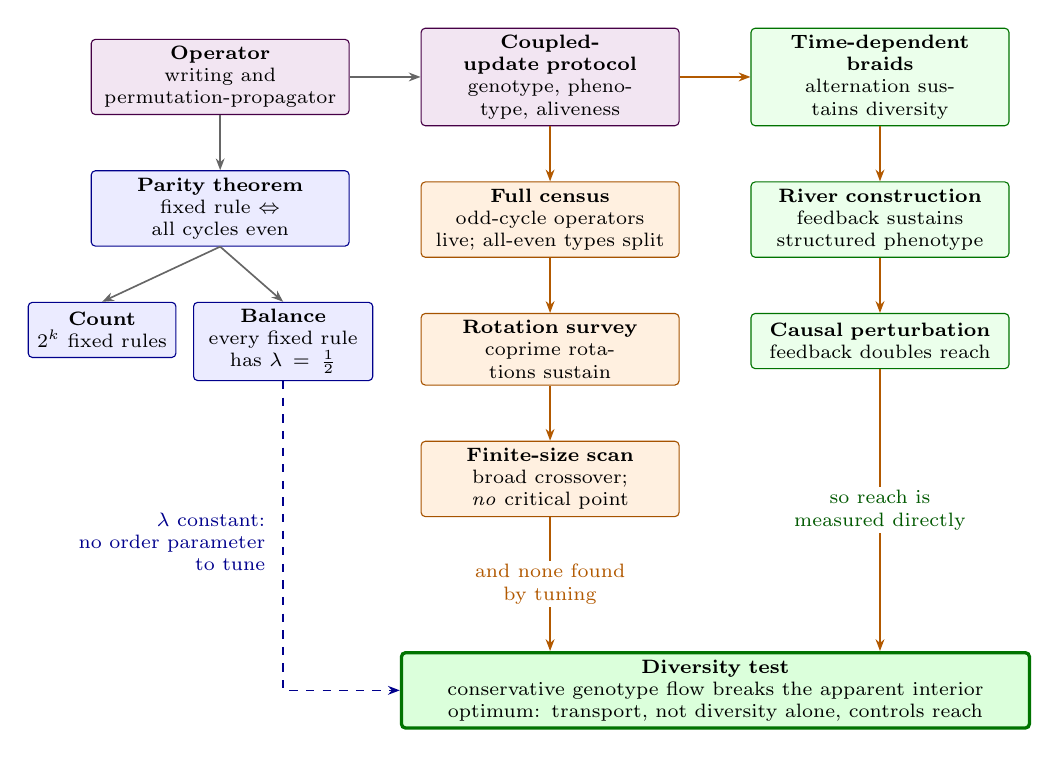
\begin{tikzpicture}[font=\scriptsize, >={Stealth[length=1.5mm]},
  bx/.style={draw, rounded corners=1.5pt, align=center, inner sep=2.5pt,
             text width=31mm, minimum height=7mm},
  defn/.style={bx, fill=violet!10, draw=violet!55!black},
  thm/.style={bx, fill=blue!8, draw=blue!55!black},
  ef/.style={bx, fill=orange!12, draw=orange!65!black},
  con/.style={bx, fill=green!8, draw=green!45!black},
  key/.style={bx, fill=green!14, draw=green!45!black, text width=78mm, very thick},
  s/.style={->, draw=black!60, semithick},
  e/.style={->, draw=orange!70!black, semithick},
  sil/.style={->, draw=blue!55!black, semithick, dashed}]
% Exact branch (left).
\node[defn] (operator) at (0,0) {\textbf{Operator}\\writing and permutation-propagator};
\node[thm,below=7mm of operator] (parity) {\textbf{Parity theorem}\\fixed rule $\Leftrightarrow$ all cycles even};
\node[thm,below=7mm of parity,xshift=8mm,text width=21mm] (balance) {\textbf{Balance}\\every fixed rule has $\lambda=\tfrac12$};
\node[thm,below=7mm of parity,xshift=-15mm,text width=17mm] (count) {\textbf{Count}\\$2^k$ fixed rules};
% Empirical branch (centre): the parameter-space reading, which returns nothing.
\node[defn,right=9mm of operator] (protocol) {\textbf{Coupled-update protocol}\\genotype, phenotype, aliveness};
\node[ef,below=7mm of protocol] (census) {\textbf{Full census}\\odd-cycle operators live; all-even types split};
\node[ef,below=7mm of census] (survey) {\textbf{Rotation survey}\\coprime rotations sustain};
\node[ef,below=7mm of survey] (crossover) {\textbf{Finite-size scan}\\broad crossover; \emph{no} critical point};
% Constructive branch (right): the dynamical reading, which finds one.
\node[con,right=9mm of protocol] (braid) {\textbf{Time-dependent braids}\\alternation sustains diversity};
\node[con,below=7mm of braid] (river) {\textbf{River construction}\\feedback sustains structured phenotype};
\node[con,below=7mm of river] (compute) {\textbf{Causal perturbation}\\feedback doubles reach};
% The result the branches converge on.
\node[key,below=17mm of crossover,xshift=21mm] (axis)
  {\textbf{Diversity test}\\conservative genotype flow breaks the apparent
   interior optimum: transport, not diversity alone, controls reach};
% Arrows show dependence, not merely reading order.
\draw[s] (operator)--(parity); \draw[s] (parity.south)--(balance.north); \draw[s] (parity.south)--(count.north);
\draw[s] (operator)--(protocol);
\draw[e] (protocol)--(census); \draw[e] (census)--(survey); \draw[e] (survey)--(crossover);
\draw[e] (protocol)--(braid);
\draw[e] (braid)--(river); \draw[e] (river)--(compute);
% The three contributions to the main finding, each labelled.
\draw[e] (crossover.south)--(crossover.south|-axis.north)
  node[midway, fill=white, inner sep=1.2pt, font=\scriptsize,
       text=orange!70!black, align=center]
  {and none found\\by tuning};
\draw[e] (compute.south)--(compute.south|-axis.north)
  node[midway, fill=white, inner sep=1.2pt, font=\scriptsize,
       text=green!35!black, align=center]
  {so reach is\\measured directly};
\draw[sil] (balance.south)|-(axis.west)
  node[pos=.26, left=1mm, font=\scriptsize, text=blue!55!black, align=right]
  {$\lambda$ constant:\\no order parameter\\to tune};
\end{tikzpicture}
\caption{\textbf{Argument map and scope boundary.} Part~I contains the exact
branch (blue) and the empirical parameter-space branch (amber) inside the
permutation core. The constant value $\lambda=1/2$ closes off that classical
coordinate there; it motivates looking elsewhere but does not entail what
follows. Part~II is the constructive branch (green): it leaves the
single-operator family, introduces time- and phenotype-dependent update
architectures, and measures causal propagation. Arrows mark dependence; the
change of object between the amber and green branches is explicit.}
\label{fig:map}
\end{figure}

\part{The Permutation Core}
\label{part:core}

\section{The Object}
\label{sec:object}

A cellular automaton normally evolves a field of \emph{states} under one
fixed rule. Here each cell also carries a \emph{rule}, and local writes evolve
that rule field alongside the phenotype. We display an elementary cellular
automaton (ECA) rule in Wolfram order,
\[
111,110,101,100,011,010,001,000,
\]
and index these displayed positions from left to right by $p=0,\ldots,7$.
Thus position $0$ is the $111$ output and most significant bit, while position
$7$ is the $000$ output and least significant bit. Throughout, the indices of
$\sig$, $w$, $g$, and $\bit{p}$ are these \emph{displayed positions}, not the
binary values of the neighbourhoods. If $n\in\{0,\ldots,7\}$ is a numerical
neighbourhood value, its rule output is therefore $g(7-n)$.

We study the operator $P_\sig$, parameterised by a permutation
$\sig\in S_8$ of the displayed positions. Writing the displayed byte as a map
$g\colon\{0,\dots,7\}\to\{0,1\}$, the operator sends $g$ to $P_\sig g$ defined by
\begin{equation}
(P_\sig\, g)(q) \;=\; \lnot\, g\bigl(\sig^{-1}(q)\bigr),
\qquad\text{equivalently}\qquad \bit{\sig(p)} := \lnot\,\bit{p}.
\label{eq:prop}
\end{equation}
Each output bit is one input bit, at the position $\sig$ moves it to, negated;
$P_\sig$ is thus a permutation of the eight coordinates composed with a global
complement. The truth table is thereby itself an eight-cell automaton whose
wiring is $\sig$ and whose update is Boolean negation --- an automaton inside
the automaton. Equation~\eqref{eq:prop} defines a family of $8! = 40{,}320$
operators that is finite, exhaustively enumerable, and, as we show below,
exactly classified.

The legacy engine stored its table in the order
$000,001,010,100,011,101,110,111$. Whenever a legacy writing is imported, the
reproduction code conjugates it into the displayed Wolfram order above before
we quote its permutation or apply names such as offset $+2$.

\begin{definition}[fold,label={def:writing}]{Writings, elementary writes, and propagators}
A \emph{writing} is any function $w\colon\{0,\dots,7\}\to\{0,\dots,7\}$ on the
truth-table positions. Its elementary update at source position $p$ is
\[
(U_{w,p}g)(q)=
\begin{cases}
\lnot g(p),&q=w(p),\\
g(q),&q\ne w(p).
\end{cases}
\]
Thus one update complements source bit $p$ and writes it to target $w(p)$. If
$w$ is a bijection---a permutation $\sig\in S_8$---all eight writes can be
performed simultaneously without collisions, giving the
\emph{permutation-propagator} $P_\sig$ in Equation~\eqref{eq:prop}. Its fixed
bytes are exactly the bytes fixed by every $U_{\sig,p}$. For a non-injective
writing, individual updates $U_{w,p}$ remain well defined, but a simultaneous
$P_w$ requires a collision-resolution convention; such a writing also has
\emph{gaps}, or positions targeted by no source.
\end{definition}

\begin{observation}[fold,label={obs:core}]{Permutations form a small bijective core}
Permutations are only the bijective core of a far larger class: there are
$8!=40{,}320$ permutations but $8^{8}=16{,}777{,}216$ writings, so the
permutations are $0.24\%$ of the whole. The cycle-structure algebra of
\secref{sec:classification} is available only on this core. The historical
operator $[0\,0\,1\,2\,3\,4\,5\,6]$ (Figure~\ref{fig:fig2pair}) is itself a
non-bijective writing---bits $0$ and $1$ both write to position $0$, and
position $7$ is never written---and its behaviour ranges widely between its two
standard-order forms.
\end{observation}

Box~\ref{box:propagator} works through one member of the
family bit by bit.

\begin{workedexample}[fold,label={box:propagator}]{A simultaneous propagator by hand}
\small
Write an ECA rule in Wolfram's standard neighbourhood order:
\begin{center}
\setlength{\tabcolsep}{3.2pt}
\begin{tabular}{c@{\quad}*{8}{c}}
position & $0$ & $1$ & $2$ & $3$ & $4$ & $5$ & $6$ & $7$ \\
neighbourhood & $111$ & $110$ & $101$ & $100$ & $011$ & $010$ & $001$ & $000$ \\
\midrule
Rule 110 & $0$ & $1$ & $1$ & $0$ & $1$ & $1$ & $1$ & $0$ \\
\end{tabular}
\end{center}
Thus Rule~110 is the byte $01101110$. Let $\sig(p)=p+2\pmod 8$ on the
displayed position indices: each source bit is complemented and written two
positions further to the right, wrapping at the end.
Carrying out the eight writes gives
\[
P_{+2}(01101110)=01100100,
\]
which is Rule~100. This changes what the cell does to its black-and-white
phenotype. For example, neighbourhood $011$ maps to $1$ under Rule~110 but
to $0$ under Rule~100. The propagator has not directly flipped a phenotype
cell; it has changed the truth table that the cell will use.
\end{workedexample}

The simultaneous operator acts on one eight-bit rule; the spatial experiments
place its elementary writes inside a two-layer automaton.

\begin{definition}[fold,label={def:genopheno}]{Genotype and phenotype}
Each cell carries an eight-bit rule. The field of rules---the
\emph{genotype}---governs a field of black-and-white states---the
\emph{phenotype}---and neighbouring rules also interact. One complete local
update (Box~\ref{box:metaca-step}) evolves both layers; this is the computation
behind the space--time diagrams in Figure~\ref{fig:regimes}.
\end{definition}

\Needspace{0.72\textheight}
\begin{workedexample}[fold,label={box:metaca-step}]{One site, one complete MetaCA step}
\small
At time $t$, site $x$ holds an eight-bit rule $g_x(t)$ and a phenotype bit
$X_x(t)$. One ordinary coupled step has three parts.
\begin{enumerate}
\item \textbf{Express the current rule.} The phenotype neighbourhood is
evaluated by the rule at its centre. With numerical neighbourhood value
$n_x(t)=4X_{x-1}(t)+2X_x(t)+X_{x+1}(t)$, its displayed position is $7-n_x(t)$:
\[
X_x(t+1)=g_x(t)\bigl(7-n_x(t)\bigr).
\]
\item \textbf{Blend neighbouring rules.} For each truth-table position $j$,
inspect the three genotype bits
$\bigl(g_{x-1}(j),g_x(j),g_{x+1}(j)\bigr)$. If the two outer bits agree, copy
their value. Thus $(0,1,0)$ blends to $0$. If they disagree, the centre rule
decides by treating the triple as one of its ECA neighbourhoods, converting
its numerical value $n$ to displayed position $7-n$ as above. The eight
coordinate-wise decisions form an intermediate rule
\[
h_x=B\bigl(g_{x-1}(t),g_x(t),g_{x+1}(t)\bigr).
\]
\item \textbf{Write one propagated bit.} Draw a source position
$K_x(t)\in\{0,\ldots,7\}$ uniformly and apply its elementary write to the
intermediate byte:
\[
g_x(t+1)=U_{\sig,K_x(t)}(h_x).
\]
\end{enumerate}
The ordinary spatial runs make one such elementary write per cell and
generation. The historical Figure~8 variant made two. By contrast,
$P_\sig$ denotes the simultaneous eight-write map classified in
\secref{sec:classification}; its fixed bytes are precisely the bytes left
unchanged by every possible elementary write.
\end{workedexample}

The substrate---a cellular automaton whose cells hold rules rather than
states---is not itself new \parencite{corneli2015search}; what we study
is the \emph{operator} of Equation~\eqref{eq:prop}, understood as an
enumerated, exactly classified family. That 2015 paper found a single
member of this family, encountered through a programming error and not
recognised as one of many; we now give the family an essentially complete
characterisation. The canonical symmetry group of ECA
rule space has order four (reflection $\times$ complement, collapsing $256$
rules to $88$ classes) \parencite{svozil2025symmetries}; it is not $S_8$,
and the negation-carrying, $\sig$-parameterised family of
Equation~\eqref{eq:prop} does not appear in it. Rule-space permutation as a
parameterised, enumerated family with a derived fixed-point structure does
not appear in the literature we have surveyed; the nearest neighbours
augment cellular automata with state-dependent feedback
\parencite{pavlic2014selfref} rather than permuting the rule itself. Two
established genres are adjacent but distinct: per-cell rules (non-uniform or
$\nu$-CA \parencite{dennunzio2011nonuniform}) and rules that change during
evolution (rule-changing or programmable CA
\parencite{mori1998rulechanging}). Non-uniform cellular automata are not, by
themselves, the source of novelty here: when each site draws its rule from a
finite set, the resulting system can be represented as a uniform cellular
automaton on a product alphabet \parencite{dennunzio2011nonuniform}. Our
contribution instead concerns the permutation-propagator family and its
fixed-point structure.

\begin{figure}[tp]
\centering
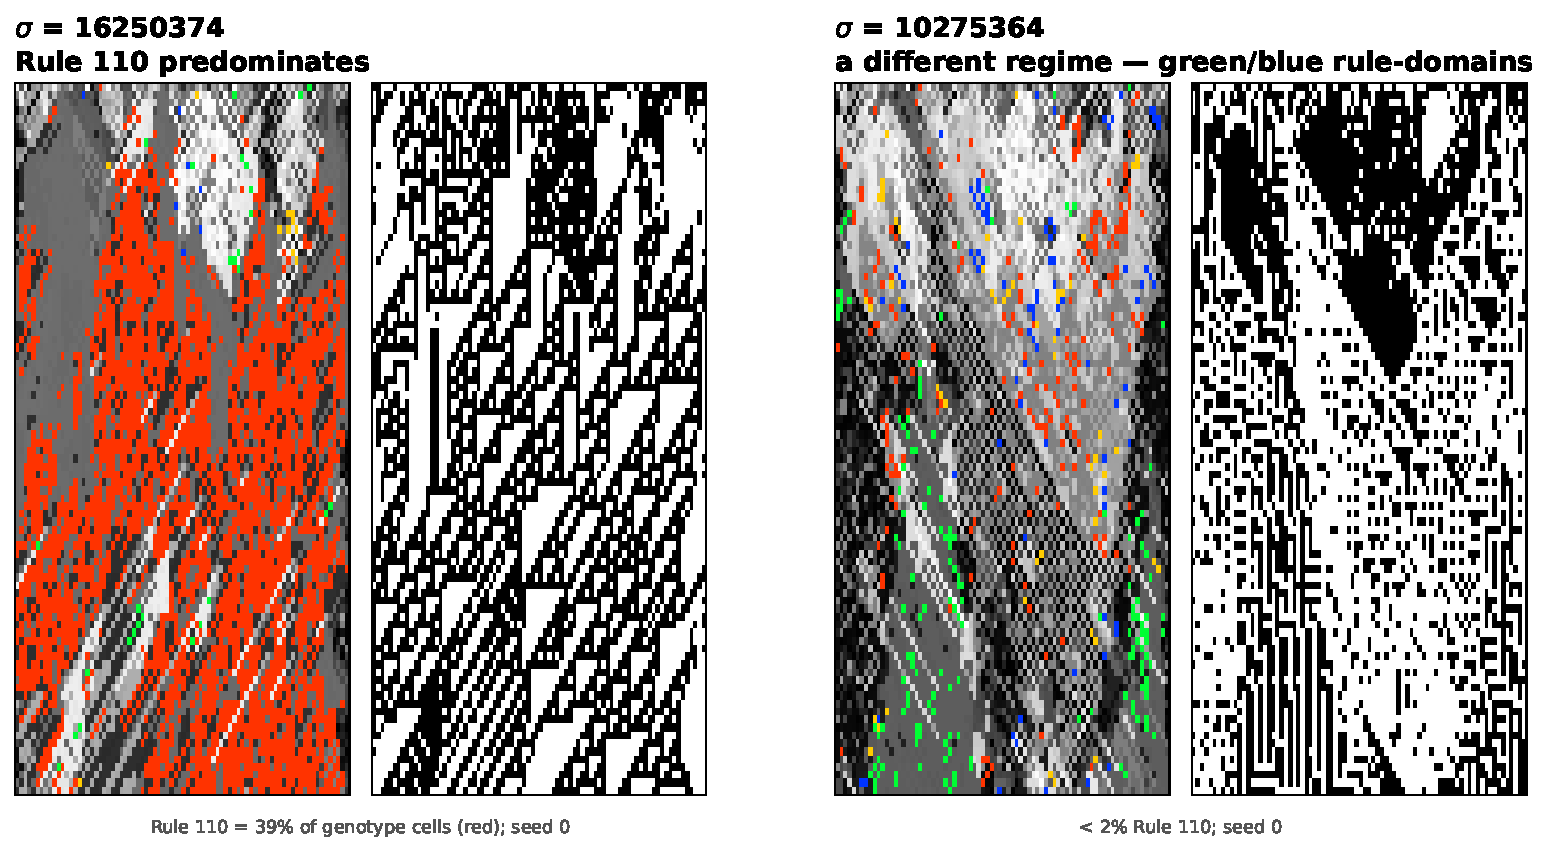
\includegraphics[width=\linewidth]{figures/rule110_spread.pdf}
\caption{Two operators from the family, each shown over time as genotype
(256-colour, left) and phenotype (black and white, right). Under
$\sig = 16250374$ the genotype field comes to be dominated by ECA
Rule~110---the red cells, $39\%$ of the genotype at the representative seed
($35\%$ over six seeds)---and the phenotype accordingly displays Rule~110's
characteristic gliders; under $\sig = 10275364$ a different regime of
rule-domains forms (green and blue, under $2\%$ Rule~110). The operator does not merely stir rule space: it
drives it toward particular, computationally distinguished rules. Genotype
colours are the legacy engine's own.}
\label{fig:regimes}
\end{figure}

\section{The Classification}
\label{sec:classification}

\subsection{Fixed points exist iff every cycle is even}

\begin{theorem}[fold,label={thm:parity}]
$P_\sig$ has a fixed point (a fixed rule) if and only if every cycle of
$\sig$ has even length. Since a one-cycle has odd length, this already
requires $\sig$ to be fixed-point-free.
\end{theorem}

\noindent A fixed rule is a $g$ invariant under~\eqref{eq:prop}, i.e.\ a
$\sig$-equivariant Boolean colouring with $g(\sig k) = \lnot\,g(k)$.
Follow a cycle of length $L$: equivariance forces
$g(k) = (\lnot)^{L} g(k)$, and $(\lnot)^{L}$ is the identity exactly when
$L$ is even; conversely, colour each orbit by the parity of its distance
from a chosen representative. A one-cycle of $\sig$ ($L=1$) is odd and so
admits no such colouring, which is why even cycles are required throughout.

Box~\ref{box:even-cycle} shows the theorem on the offset-$+2$ operator. The
same small calculation also makes the later $2^k$ count and forced
$\lambda=1/2$ balance visible before we state them generally.

\begin{workedexample}[fold,label={box:even-cycle}]{Even and odd cycles}
\small
For offset $+2$ on eight truth-table positions,
\[
\sig=(0\;2\;4\;6)(1\;3\;5\;7).
\]
A fixed rule must change colour at every arrow because
$g(\sig k)=\lnot g(k)$. Around either four-cycle it can therefore read
$0101$ or $1010$: after four negations it returns consistently to its
starting bit. The two four-cycles are coloured independently, so two binary
choices fix all eight truth-table entries $\bit{0},\dots,\bit{7}$. Read back as
an ECA rule number---those eight bits in Wolfram neighbourhood order (the table
of \secref{sec:object}) taken as an integer in $0$--$255$---the four colourings
are the fixed rules
\[
2^2=4:\quad
51,\ 102,\ 153,\ 204,
\]
each with four zero-bits and four one-bits. An odd cycle admits no such
colouring: after an odd number of negations the bit returns to its starting
position demanding its own opposite, so no fixed rule exists. Admitting a fixed
rule and settling onto one are distinct. An operator carrying an odd cycle has no
fixed rule for its field to collapse onto, and its field correspondingly stays
diverse (the any-odd reduced rotate$+2$, Figure~\ref{fig:parity}, right); whether
a fixed-point-bearing operator collapses onto one of its fixed rules is a
separate, dynamical question (\secref{sec:interrupter}).
\end{workedexample}

This is the signed-cycle fixed-point theorem of Boolean-network theory
\parencite{aracena2008maximum} specialised to~\eqref{eq:prop}: our operator
is a Boolean network whose signed interaction digraph is $\sig$ with every
arc negative, a negation-cycle of length $\ell$ has sign $(-1)^\ell$, and
an isolated negative cycle admits no fixed point while a positive (even)
one admits exactly two. We contribute a machine-checked proof of the
specialised statement in Lean~4 / Mathlib.\footnote{%
\texttt{DarkTower/Patterns/Propagator.lean}, theorem
\texttt{hasAlternatingColouring\_iff\_cycleType\_even}; \texttt{lake build}
clean, no \texttt{sorry} or \texttt{axiom}.}

\subsection{The closed form}

The number of $\sig \in S_{2n}$ with all cycles even is $((2n-1)!!)^2$, with
exponential generating function $\sum_n ((2n-1)!!)^2 x^{2n}/(2n)! =
1/\sqrt{1-x^2}$ (the ``set of even cycles'' construction).
For $S_8$ this is $105^2 = 11{,}025$ of $40{,}320$, or $27.34\%$. The count
is classical: it is \textcite{oeis_a001818} and appears as
\textcite[Problem~5.34(c)]{stanley1999enumerative} and in
\textcite{riordan1968combinatorial}. We claim it only as the enumeration of
our operator family, not as a new identity.

\subsection{Fixed bytes number \texorpdfstring{$2^k$}{2 to the k}}

\begin{corollary}[fold,label={cor:count}]
An all-even $\sig$ with $k$ cycles has exactly $2^k$ fixed bytes; any $\sig$ with
an odd cycle has none.
\end{corollary}
Each even cycle admits exactly two alternating colourings, chosen independently
across cycles, whence $2^k$; the zero case is Theorem~\ref{thm:parity}. This too
is machine-checked.%
\footnote{\texttt{alternatingColouring\_card\_eq\_two\_pow\_cycleType\_card}.}
Summed against these weights the family is consistent:
$\sum 2^{k}$ over all-even $\sig$ equals $(2n)! = 8! = 40{,}320$, the total
number of fixed bytes across the family.

\section{Every Fixed Point Is Balanced}
\label{sec:lambda}

\begin{definition}[fold,label={def:lambda}]{Langton's activity $\lambda$}
$\lambda$ measures a rule's \emph{activity}: the fraction of its neighbourhood
entries that map to the non-quiescent
state~\parencite{langton1990computation}---for an eight-bit ECA table, the
Hamming weight over eight, $\lambda = \lVert r \rVert_1 / 8$, from $0$ (every
neighbourhood dies) through $1/2$ to $1$. A rule with $\lambda = 1/2$ is
\emph{balanced}.
\end{definition}

\begin{observation}[fold,label={obs:lambda}]{Balance is a truth-table property}
Langton's thesis was that complex behaviour concentrates near a critical
$\lambda$, shown most clearly for larger tables ($K=4$, $N=5$); for the
two-symbol, three-neighbour ECAs Langton is explicit that $\lambda$ only roughly
correlates with dynamics, and later work is
cautious~\parencite{mitchell1993revisiting}. Theorem~\ref{thm:lambda} below
concerns the \emph{value} $\lambda = 1/2$ itself---balance---which we keep
separate from any empirical claim about what it predicts dynamically.
\end{observation}

\subsection{Every fixed point has \texorpdfstring{$\lambda = 1/2$}{lambda = 1/2}}

\begin{theorem}[fold,label={thm:lambda}]
Every fixed point of every operator in the family has exactly four one-bits;
equivalently, Langton's activity parameter $\lambda = 4/8 = 1/2$.
\end{theorem}

\noindent By Theorem~\ref{thm:parity} each cycle has even length $2m$; an
alternating colouring assigns such a cycle exactly $m$ ones; summing over
cycles gives $(\sum L)/2 = 8/2 = 4$. Exhaustive enumeration confirms it:
across all $40{,}320$ operators and all their fixed points, every one has
Hamming weight four, with zero exceptions. The statement is machine-checked
for $\mathrm{Fin}\,8$.\footnote{%
\texttt{alternatingColouring\_true\_card\_eq\_four}: the true-cells and
false-cells are put in bijection by $\sig$, forcing each to number four.}

We are deliberate about the standing of this result. Langton's critical
value was obtained empirically, as a statistic over rule space
\parencite{langton1990computation}, and its status as an order parameter
was contested: \textcite{mitchell1993revisiting} refuted
\textcite{packard1988adaptation}'s specific genetic-algorithm clustering
claim, not the definition of $\lambda$, which survived as one axis among
others such as Wuensche's $Z$ \parencite{wuensche1999classifying}. There is
a folklore intuition for why $1/2$ is special --- binomial sampling variance
$\lambda(1-\lambda)$ is maximal there --- and it is not ours; and it has been
noted that $\lambda$ alone does not fix a rule's dynamical class, distinct
classes coexisting at a single value \parencite{sakai2002edge}. What
Theorem~\ref{thm:lambda} adds is narrower and firmer than any of these: under
the complementation in~\eqref{eq:prop} the value $1/2$ is \emph{forced} as an
algebraic matter, because any alternation-under-complement colouring is
balanced by parity. We claim balance, exactly; any connection of that
balance to dynamical behaviour we treat as interpretation, not as part of the
theorem.

\subsection{The cast: which rules survive, and how many}

Under an all-even $\sig$, the fixed points of $P_\sig$---the rules it maps to
themselves---number $2^k$, where $k$ is the number of cycles of $\sig$
(\secref{sec:classification}): each even cycle admits two alternating
colourings, chosen independently across cycles. In the spatial runs these are
the rules onto which the field is observed to settle. Every one has
$\lambda = 1/2$ (Theorem~\ref{thm:lambda}), so the observed terminal
population is a cast of \emph{distinct} rules---distinct truth tables---sharing
a \emph{single} activity.

The smallest nontrivial case of the count is a single cycle, $k = 1$: two
survivors. The 2015 paper's Figure~8 already exhibited a two-rule residual: a
random field of tens of distinct rules dies off to an alternating population of
just two, rules $42$ and $170$.
Fittingly, the programming error that produced the family is what pins its
residual at two---the erroneous mutation froze a bit, splitting the field
into the cells that can reach $42$ and those that can reach $170$---so the
phenomenon was on the page before the $2^k$ count explained it.

That die-off curve---the count of distinct rules present over time---is a
natural population-level companion to $\lambda$. Where $\lambda$ is a scalar
assigned to a single rule, this curve is a property of the whole field's
trajectory; and where $\lambda$ is uninformative here---every fixed point
sits at $1/2$---the curve still varies, because it measures the population
rather than the point. We use it cautiously, as an observable rather than an
established order parameter, to tell the rotations whose fields stay diverse
from those whose fields collapse (\secref{sec:interrupter},
Figure~\ref{fig:lambda}).

Diversity of the observed population and singularity of its activity thus
coexist; the metric measures we tried do not separate the two
(\secref{sec:metrics}).

\begin{figure}[t]
\centering
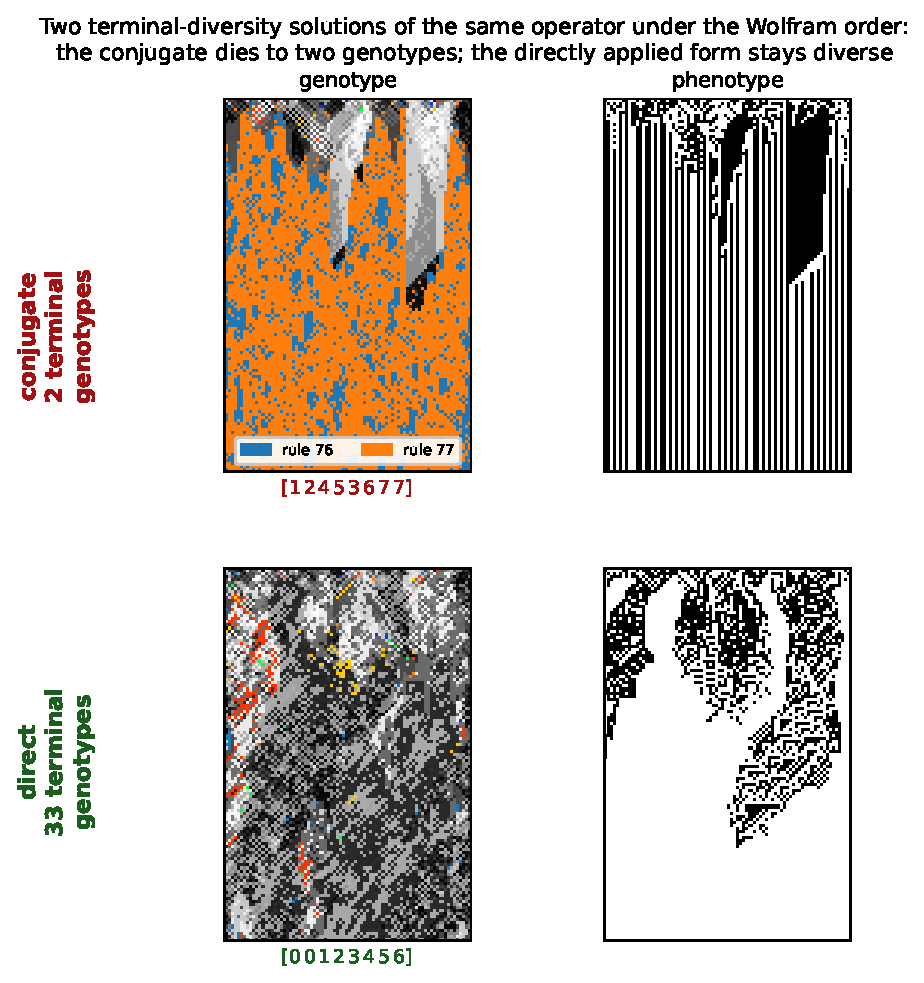
\includegraphics[width=0.82\linewidth]{figures/fig2pair.pdf}
\caption{\textbf{Two terminal-diversity solutions of one historical operator.} The
historical write $[0\,0\,1\,2\,3\,4\,5\,6]$ has two forms under the standard
Wolfram order. Its \emph{conjugate} $[1\,2\,4\,5\,3\,6\,7\,7]$ (top) reproduces the
two-rule behaviour: the genotype collapses to exactly two terminal rules---76 and 77,
adjacent, differing in a single bit---regardless of seed, while the phenotype stays
regular. Applied \emph{directly} (bottom), the same operator keeps a diverse
genotype (${\sim}30$ terminal rules). Two ends of genotypic
aliveness from one historical write.}
\label{fig:fig2pair}
\end{figure}

\subsection{A dead genotype can carry a live phenotype}
\label{sec:shell}

The balanced shell is a definite object: exactly $\binom{8}{4} = 70$ rules
carry four active outputs, and by Theorem~\ref{thm:lambda} the absorbing set of
every operator in the family lies wholly inside it. Collapse is therefore not
merely a loss of diversity but a fall onto this particular $70$-rule balanced
shell at $\lambda = 1/2$.

Balance is necessary for a genotype to freeze and silent about what the frozen
rule then does. Run each of the $70$ as an ordinary elementary CA and they
split: $32$ are phenotypically live---sustained change under iteration, the
additive rules $90$, $105$, $150$ and the class-IV rule $54$ among them---while
the rest fall quiescent. The two halves share a single $\lambda$; this is,
inside our family and by construction rather than by survey, the coexistence of
dynamical classes at one activity value that has long been urged against
$\lambda$ as an order parameter \parencite{sakai2002edge}. A field can thus die
in its genotype while the surviving rule keeps its phenotype in motion.

Figure~\ref{fig:shell} is such a field, built to specification. To seat a
collapse on a chosen live rule $R$ it suffices to pair $R$'s four active
positions with its four inactive ones as an involution: four transpositions, an
all-even operator that holds $R$ among its fixed points (Theorem~\ref{thm:parity}).
Whether the field actually settles onto that fixed rule is a separate, dynamical
question (as \secref{sec:interrupter} stresses); here it does. Carried out for
Rule~$54$ this yields
$\sig = [2\,3\,0\,1\,5\,4\,7\,6]$; run from a random field it drives the
genotype to near-uniformity---two rules survive---while the phenotype never
settles. The field has died onto Rule~$105$, another live tenant of the same
shell, whose additive dynamics keep the black-and-white panel full of
structure. Genotypic death and phenotypic death are not the same event.

One caveat marks the open edge of this. An involution fixes not its target
alone but the whole shell compatible with its pairing, and which tenant a
random field actually reaches is set by the basins, not by the construction: we
aimed at $54$ and the dynamics preferred $105$. Existence is settled---live
survivors are constructible---but \emph{steering} a field onto a named rule is
not, and is the natural next question.

\begin{figure}[t]
\centering
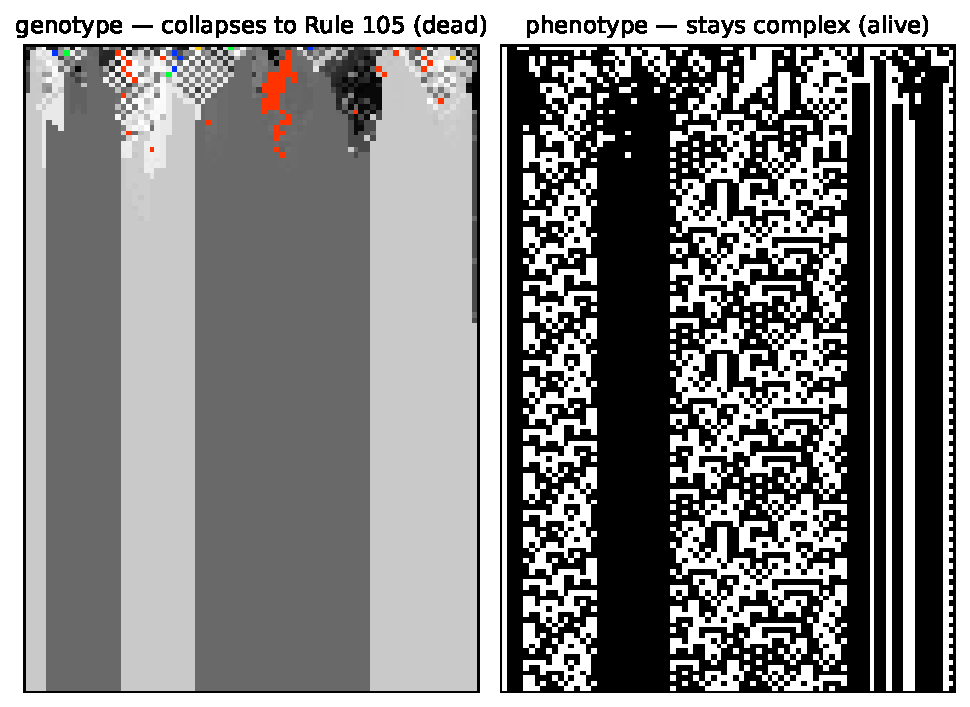
\includegraphics[width=0.82\linewidth]{figures/critical_shell.pdf}
\caption{A genotypically dead, phenotypically live field. The all-even operator
$\sig = [2\,3\,0\,1\,5\,4\,7\,6]$, built to fix the balanced shell containing
Rule~$105$, collapses the genotype (left, 256-colour) to near-uniformity within
a few dozen rows---two rules survive---yet the phenotype (right) never settles:
the field has died onto Rule~$105$, an additive $\lambda = 1/2$ rule whose
dynamics keep it complex. Seed~$1$, $W = 80$, $T = 120$.}
\label{fig:shell}
\end{figure}

\section{The Census}
\label{sec:census}

\subsection{The parity dichotomy in the spatial dynamics}

Theorems~\ref{thm:parity}--\ref{thm:lambda} concern fixed bytes; the spatial
dynamics adds stochastic elementary writes and, in the census, neighbour
blending. Figure~\ref{fig:parity} shows why fixed-point existence is not itself
a dynamical verdict: without blending, all-even rotate$+2$ settles within the
run while all-even rotate$+1$ remains diverse; the odd-cycle examples, which
lack fixed bytes, also remain diverse. The full census below
(\secref{sec:full-census}) makes this quantitative over all $40{,}320$ operators
(Table~\ref{tab:census}); the dynamical content is the \emph{death-rate
difference} between the classes, not the class sizes.

\begin{figure}[t]
\centering
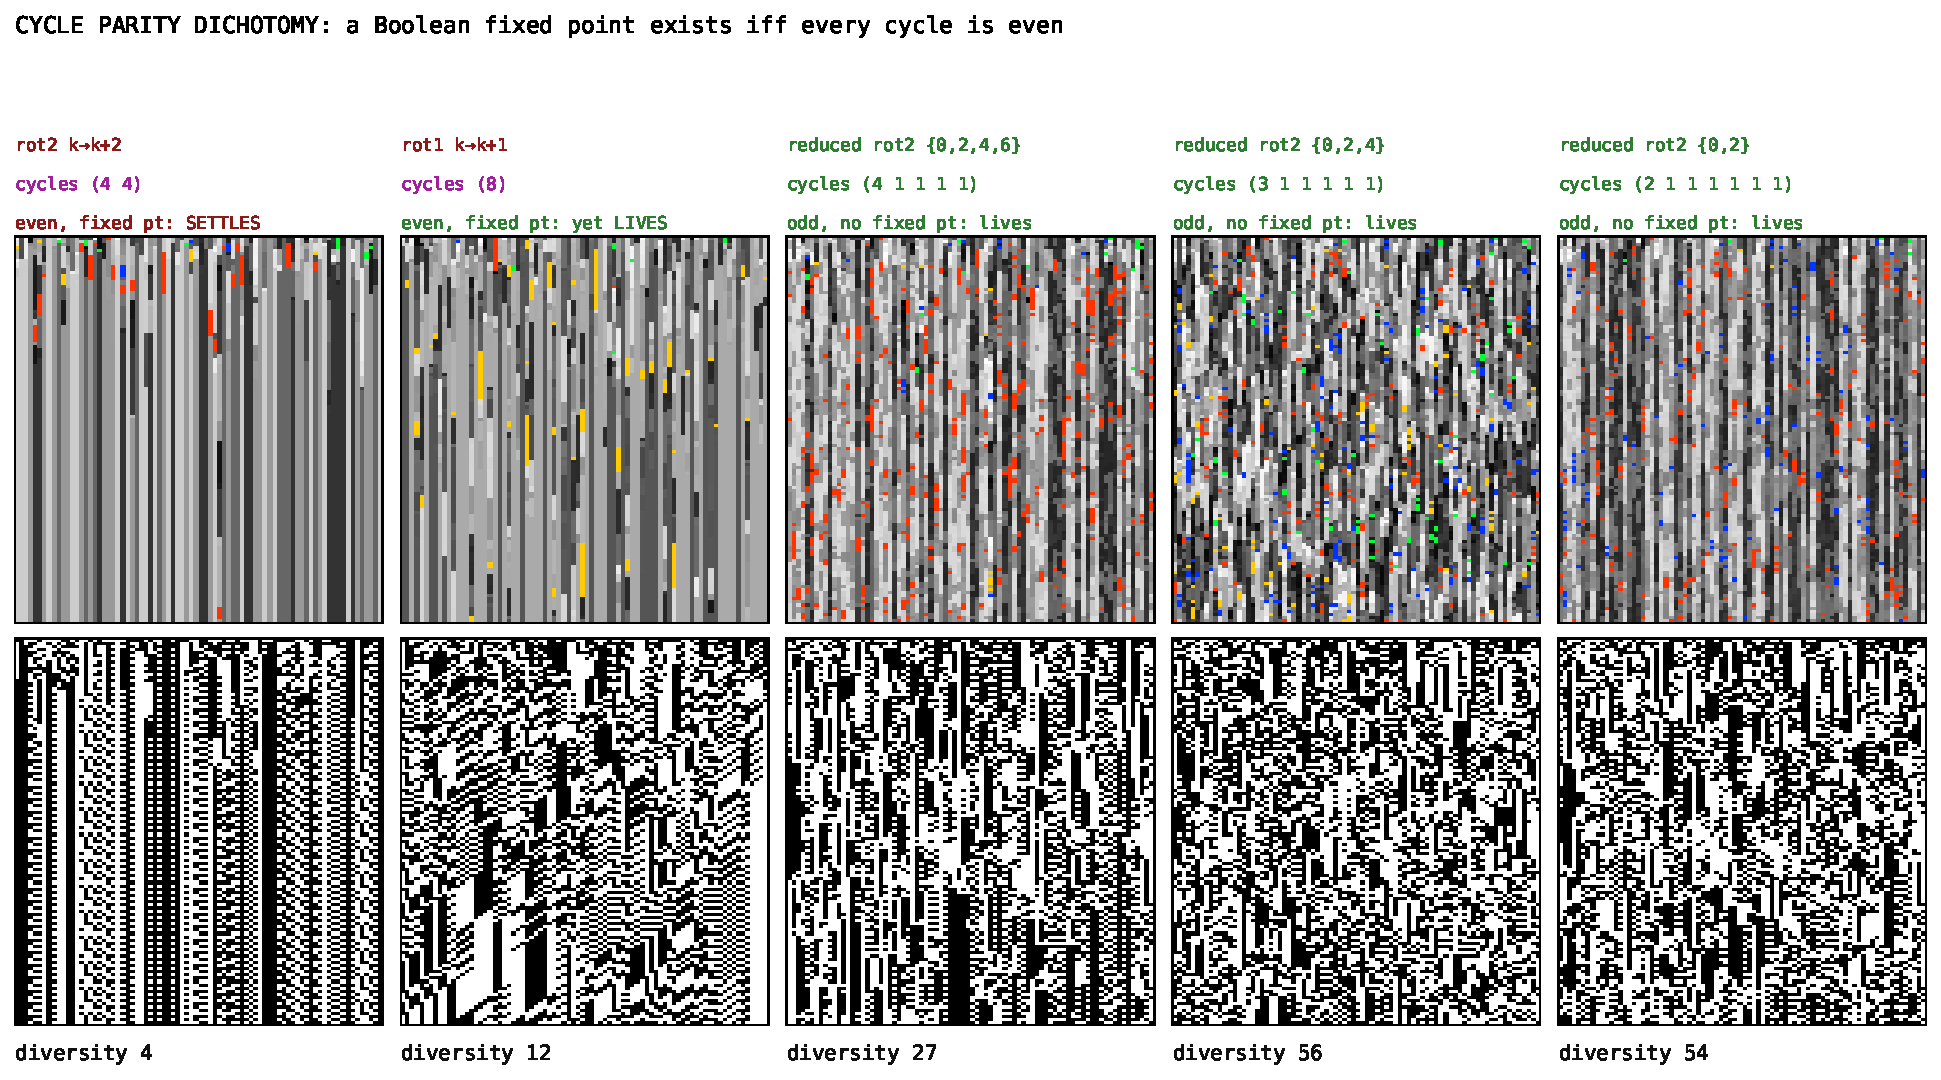
\includegraphics[width=\linewidth]{figures/parity-dichotomy.pdf}
\caption{The parity dichotomy, by example (the census of all $40{,}320$
permutations is summarised in the text). Five operators as genotype (top) and
phenotype (bottom) over time. \emph{Left:} both all-even operators possess fixed
bytes (Theorem~\ref{thm:parity}), but only rotate$+2$ settles within the run,
reaching its $2^k=2^2$ fixed rules; the single-8-cycle rotate$+1$ remains active
at diversity $12$. \emph{Right:} the odd-cycle operators
(reduced rotate$+2$, acting on a subset so the remaining positions are odd
one-cycles) possess no fixed byte and stay diverse in these runs. All five use
stochastic elementary writes without neighbour blending. The figure therefore
illustrates the theorem's fixed-byte classification while also showing that
all-even parity makes settling possible, not inevitable on a finite horizon.}
\label{fig:parity}
\end{figure}

\subsection{A prospective test: reduced \texorpdfstring{rotate$+2$}{rotate+2}}

To guard against reading structure into a completed enumeration, we fixed a
prediction before running the case. The reduced $\text{rotate}{+}2$
operators act as a single even cycle on a subset of positions and leave the
remaining positions as one-cycles; by that leftover they are \emph{not}
all-even, so by Theorem~\ref{thm:parity} they possess no fixed point and
should fall on the no-fixed-points side of the dichotomy---no rule for the
field to settle onto, and correspondingly less extinction. They do
(Figure~\ref{fig:parity}, right): they stay diverse rather than dying off.
Absence of fixed points forbids settling onto a single rule; it does not
forbid short-period behaviour, and we claim only the observed persistence of
diversity, not literal aperiodicity.

\subsection{The full census, tabulated by class}
\label{sec:full-census}

\begin{definition}[fold,label={def:aliveness}]{Census protocol and aliveness}
For each of the $40{,}320$ permutations, we ran seeds $0$--$2$ on a width-$60$
line for $100$ generations. Initial rule bytes are independent uniform draws
from $0$--$255$, initial phenotype bits are independent fair binary draws, and
both layers have fixed zero boundaries. Each genotype update uses the
neighbour blend and one uniformly sampled elementary write described in
Box~\ref{box:metaca-step}. A layer's \emph{change rate} is the mean fraction of
cells differing between consecutive rows over the final $40$ generations,
averaged over the three seeds. The layer is \emph{alive} when this rate is at
least $0.10$ and \emph{dead} otherwise. Scoring genotype and phenotype
separately gives four regimes: live/live, live/dead, dead/live, and dead/dead.
\end{definition}

The trend becomes an exhaustive finite-run observation once every operator is tabulated. We ran all
$40{,}320$ permutation-propagators and grouped them by cycle type
(Table~\ref{tab:census}).

\suppfinding{1}{The full permutation census}

\begin{table}[t]
\centering\small
\caption{Genotype-alive fraction by cycle type under the census protocol, over
all $40{,}320$ permutations. Any odd cycle forbids a fixed byte
(Theorem~\ref{thm:parity}); empirically, every such operator is alive. The
all-even types split, with collapse becoming more frequent as the number of
cycles $k$ increases.}
\label{tab:census}
\begin{tabular}{lrr}
\toprule
cycle type & count & genotype-alive \\
\midrule
any type with an odd cycle (17 types) & $29{,}295$ & $100.0\%$ \\
$[8]$        & $5{,}040$ & $82.9\%$ \\
$[2\,6]$     & $3{,}360$ & $70.0\%$ \\
$[4\,4]$     & $1{,}260$ & $66.7\%$ \\
$[2\,2\,4]$  & $1{,}260$ & $49.2\%$ \\
$[2\,2\,2\,2]$ & $105$   & $25.7\%$ \\
\bottomrule
\end{tabular}
\end{table}

\section{Fixed Points Are Not Attractors}
\label{sec:interrupter}

\begin{figure}[p]
\centering
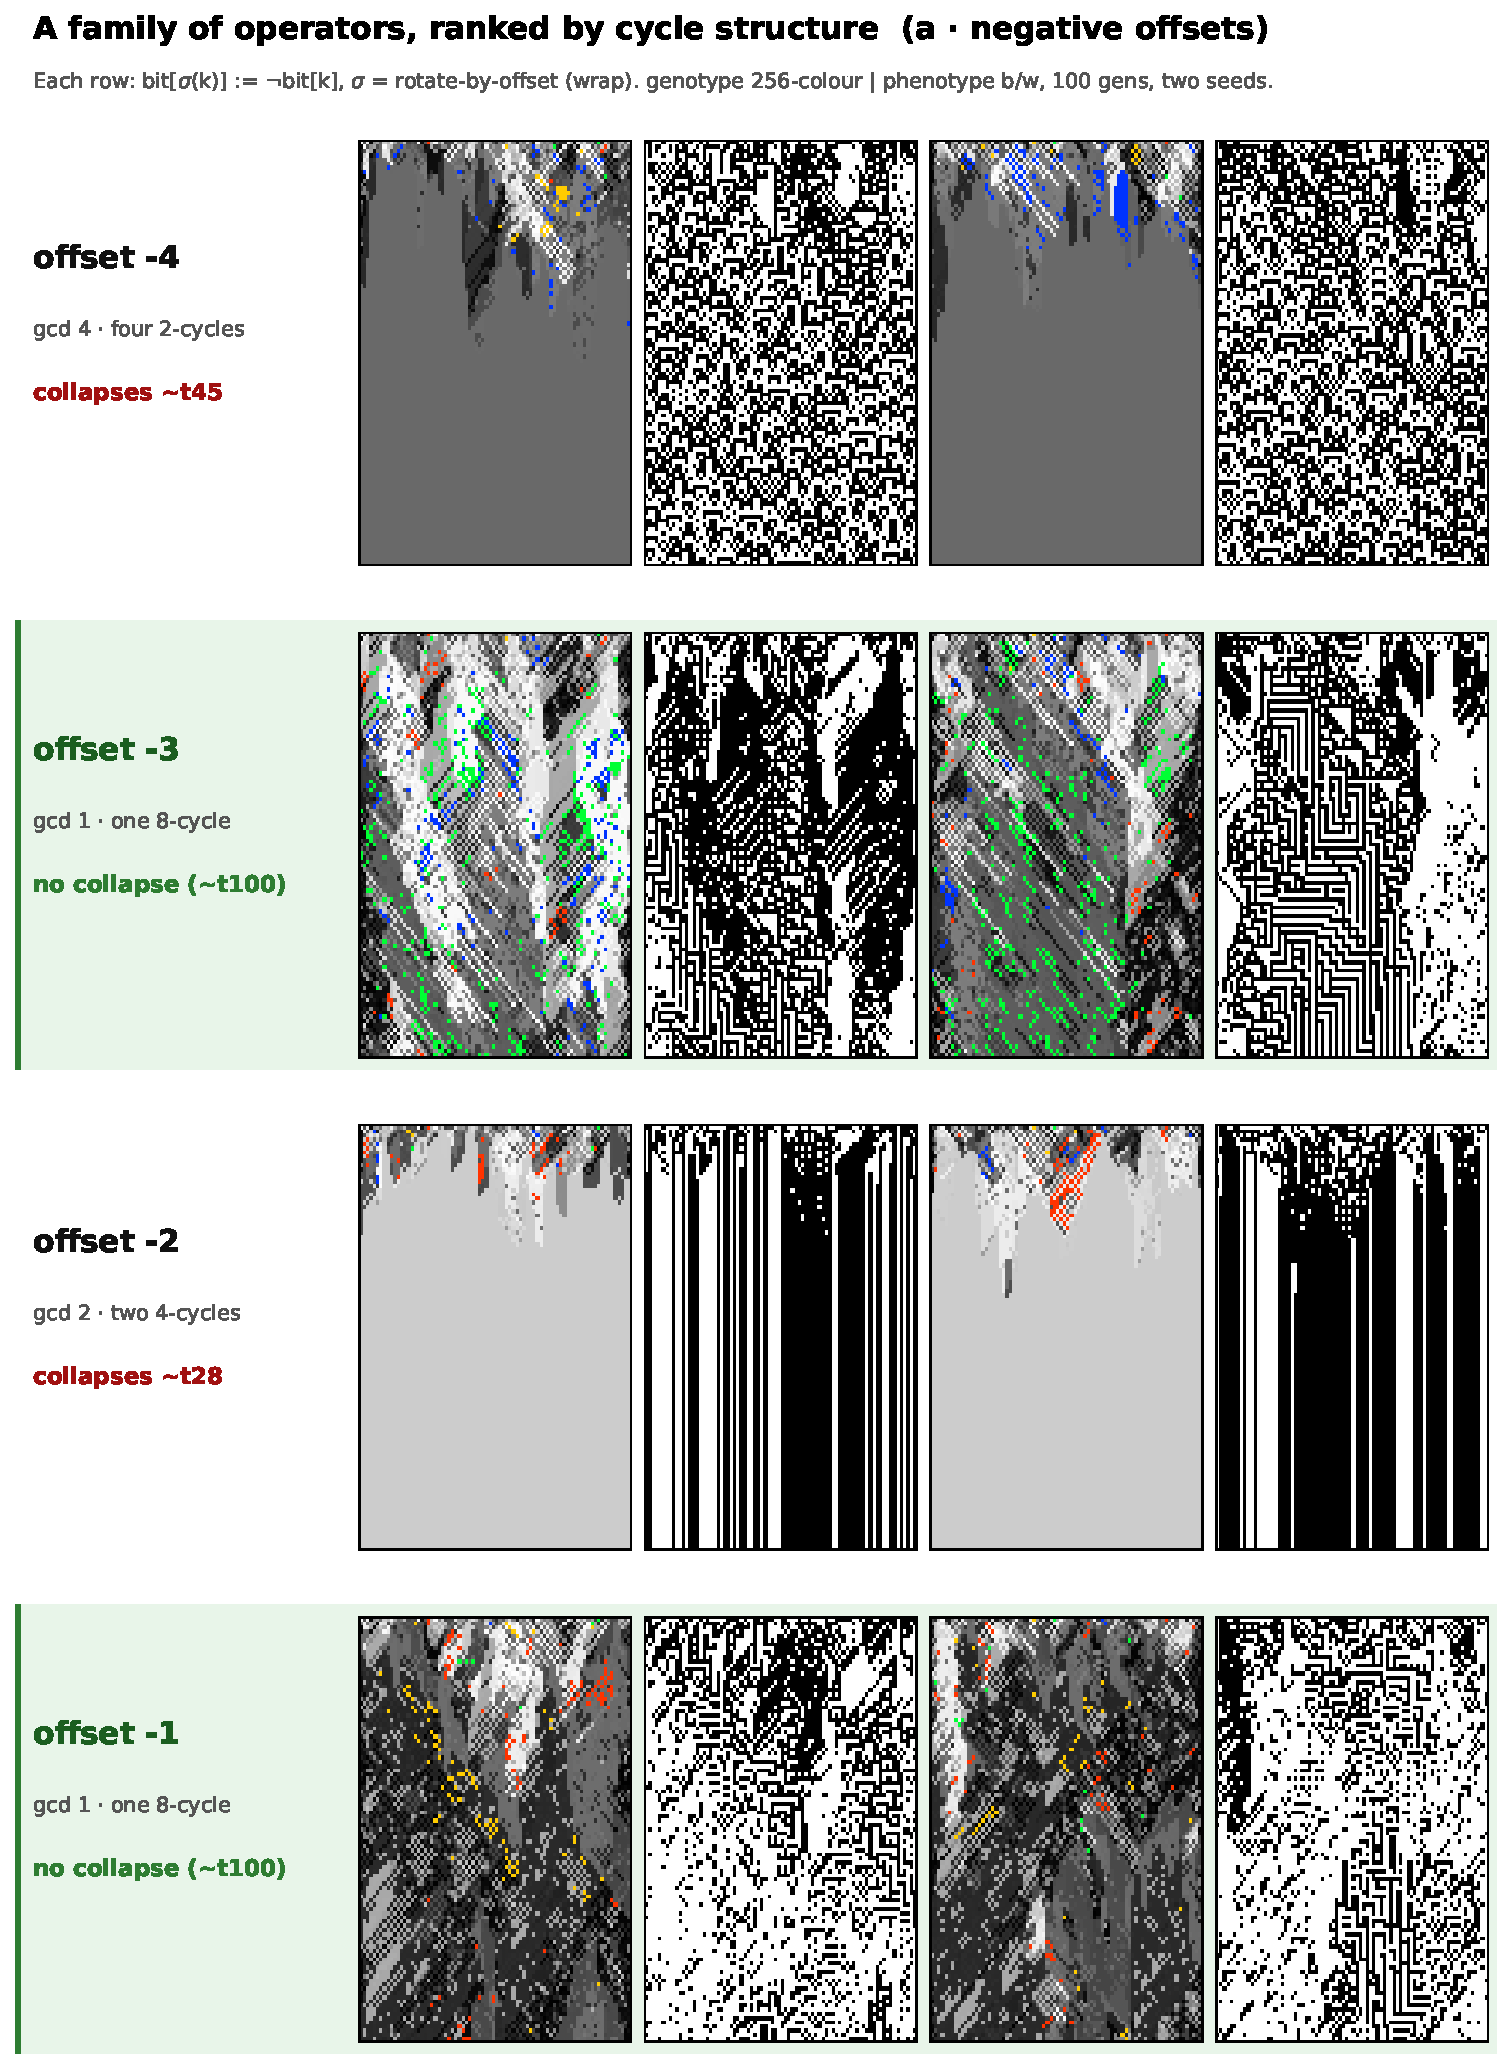
\includegraphics[height=0.73\textheight]{figures/survey_a.pdf}
\caption{\textbf{(a)~Negative offsets.} The rotation subfamily, ordered by
offset: each row is one wrap rotation $\bit{\sig(k)} := \lnot\,\bit{k}$ (two
seeds; genotype in 256 colours, phenotype black and white, first hundred
generations). Of these all-even rotations only the single 8-cycles,
$\gcd(\text{offset},8) = 1$---offset $\pm 1$ and $\pm 3$, highlighted---sustain a
high-diversity phase; offset $\pm 2$ ($\gcd 2$) and $\pm 4$ ($\gcd 4$) collapse.
See Worked Example~\ref{box:survey}; continued in~(b).}
\label{fig:eoc}
\end{figure}

\begin{figure}[p]
\ContinuedFloat
\centering
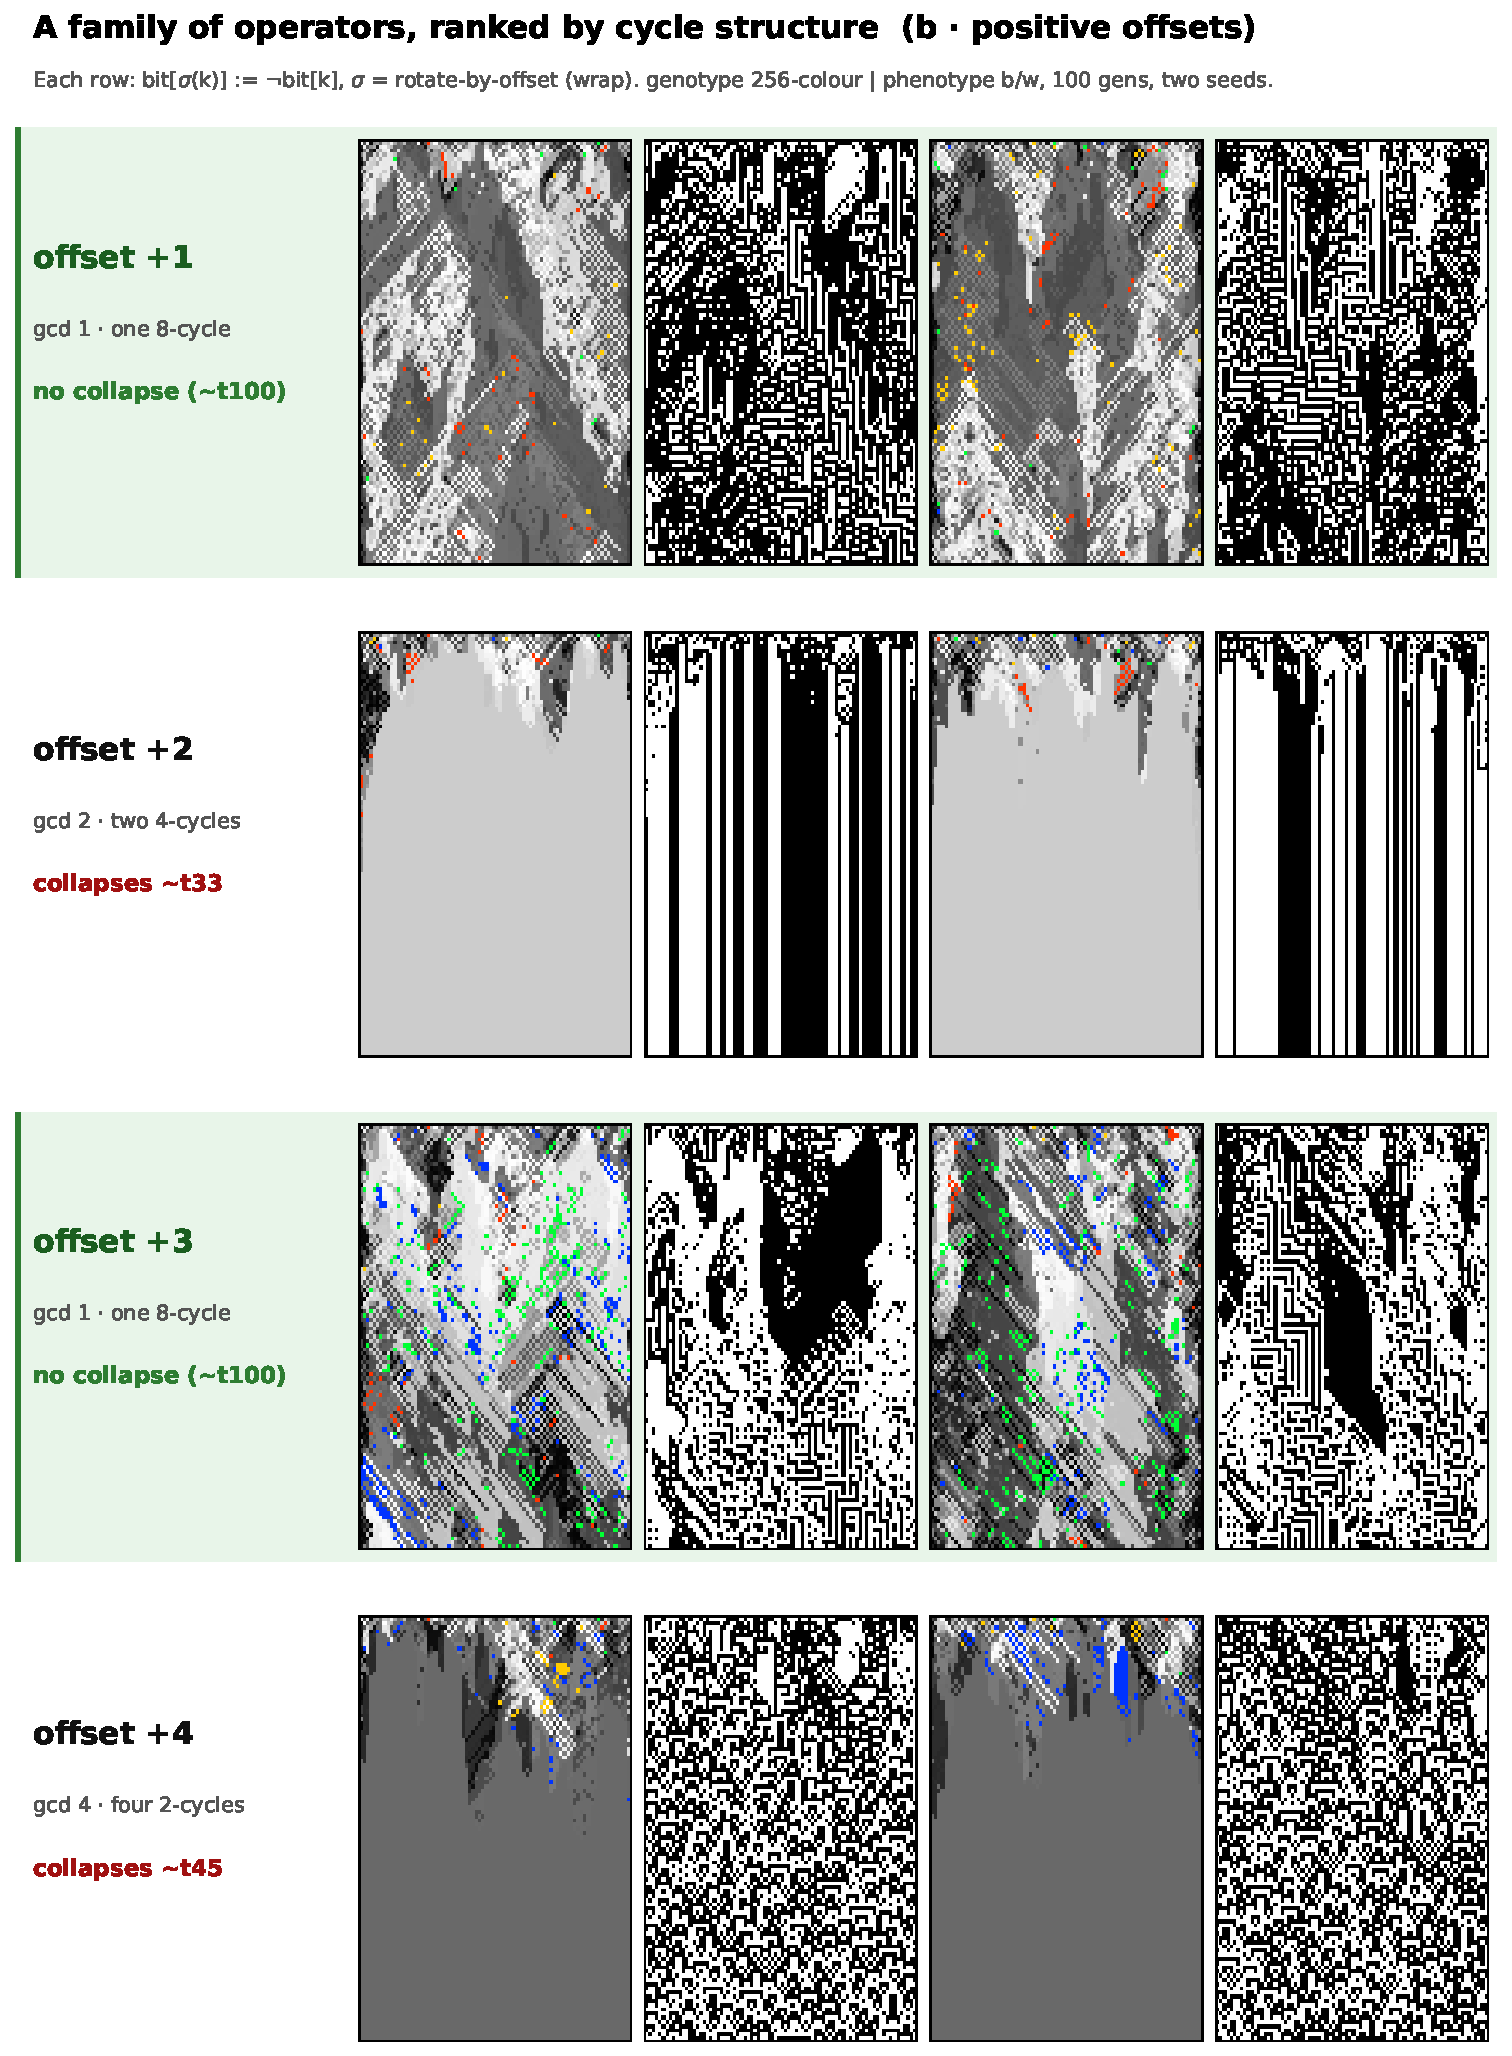
\includegraphics[height=0.73\textheight]{figures/survey_b.pdf}
\caption{\textbf{(b)~Positive offsets.} Continued from~(a). The classification is
symmetric under $d \to -d$ (verdict follows $\gcd(d,8)$), so offset $+1$ sustains
as offset $-1$ does, and offset $+2$ collapses as offset $-2$ does---inverse
rotations sharing verdict but not their transients (Worked
Example~\ref{box:survey}). Possessing a fixed point and staying near it are
different properties: the two pages visually summarise the distinction between
fixed-point existence and spatial persistence.}
\end{figure}

\begin{workedexample}[fold,label={box:survey},breakable=false]{Reading the rotation survey}
\small
The fields of Figure~\ref{fig:eoc} evolve under the \emph{spatially coupled}
dynamics of \secref{sec:interrupter}---stochastic elementary writes together
with the coupling between cells---not $P_\sig$ applied cell-by-cell. This is
what the survey turns on. Without the blend, Figure~\ref{fig:parity} already
shows rotate$+1$ remaining active over the observed horizon while rotate$+2$
settles. With neighbour blending, the finite-horizon split persists and widens:
the single 8-cycles---$\gcd(\text{offset},8)=1$, offset $\pm 1$ and $\pm 3$---
sustain a high-diversity field, while offset $\pm 2$ ($\gcd 2$) and $\pm 4$
($\gcd 4$) collapse; that split is what the survey shows.

The two panels are \emph{almost} mirror images, and where they differ is
instructive. Offset $+d$ and offset $-d$ are the same permutation exactly when
$2d \equiv 0 \pmod 8$---so offset $\pm 4$ (and the identity) are one operator with
bit-identical panels, whereas offset $\pm 1$ and $\pm 3$ are distinct
\emph{inverse} rotations. Inverses share cycle structure, fixed rules, and the
sustain-or-collapse verdict, but not their transient dynamics: offset $+1$ and
offset $-1$ realise the same sustaining regime through visibly different fields.
\end{workedexample}

Possessing a fixed point (Theorem~\ref{thm:parity}) is not the same as
reaching one, and $P_\sig$ does not by itself move a rule toward
$\lambda = 1/2$. Because $P_\sig$ complements every bit,
$\lambda(P_\sig g) = 1 - \lambda(g)$: the operator \emph{reflects} activity
across $1/2$, exactly preserving the distance $\lvert\lambda - 1/2\rvert$
rather than contracting toward it. And because $P_\sig$ is a bijection on
bytes, a generic rule lies on a periodic orbit and simply cycles---its fixed
points are fixed, but they are not attractors and have no basins. The only
rules pinned at $\lambda = 1/2$ are the fixed points themselves. Attraction in
the experiments therefore belongs to the stochastic elementary-write dynamics,
with or without neighbour coupling, rather than to iteration of the simultaneous
map $P_\sig$.

\suppfinding{2}{The rotation survey}

\begin{figure}[t]
\centering
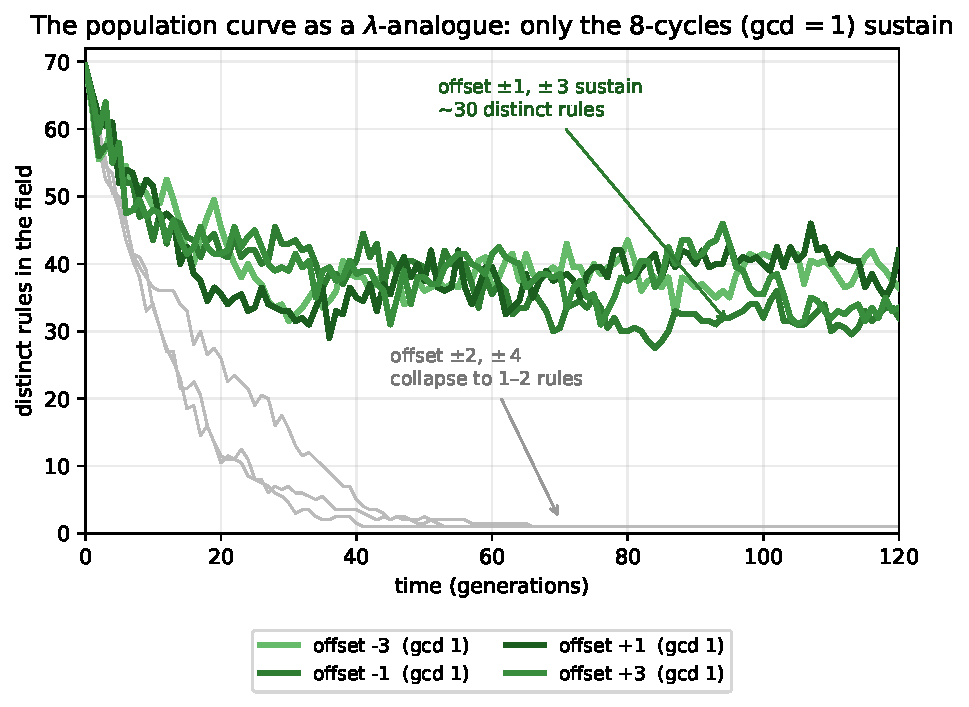
\includegraphics[width=\linewidth]{figures/lambda_analogue.pdf}
\caption{A population observable: distinct rules in the field over time, for
the wrap rotations (two seeds each). All begin at $\approx 70$; the four
8-cycles, $\gcd(\text{offset},8)=1$ (offset $\pm 1$ and $\pm 3$, green), keep a
large diverse population, while offset $\pm 2$ and $\pm 4$ (grey) collapse to one
or two rules. This makes quantitative, on the runs shown, the difference visible
by eye in Figure~\ref{fig:eoc}. Figure~\ref{fig:parity} gives the corresponding
without-blend comparison for offsets $+1$ and $+2$: the former remains active at
lower diversity over that run, while the latter settles onto its four fixed
rules.}
\label{fig:lambda}
\end{figure}

\begin{figure}[t]
\centering
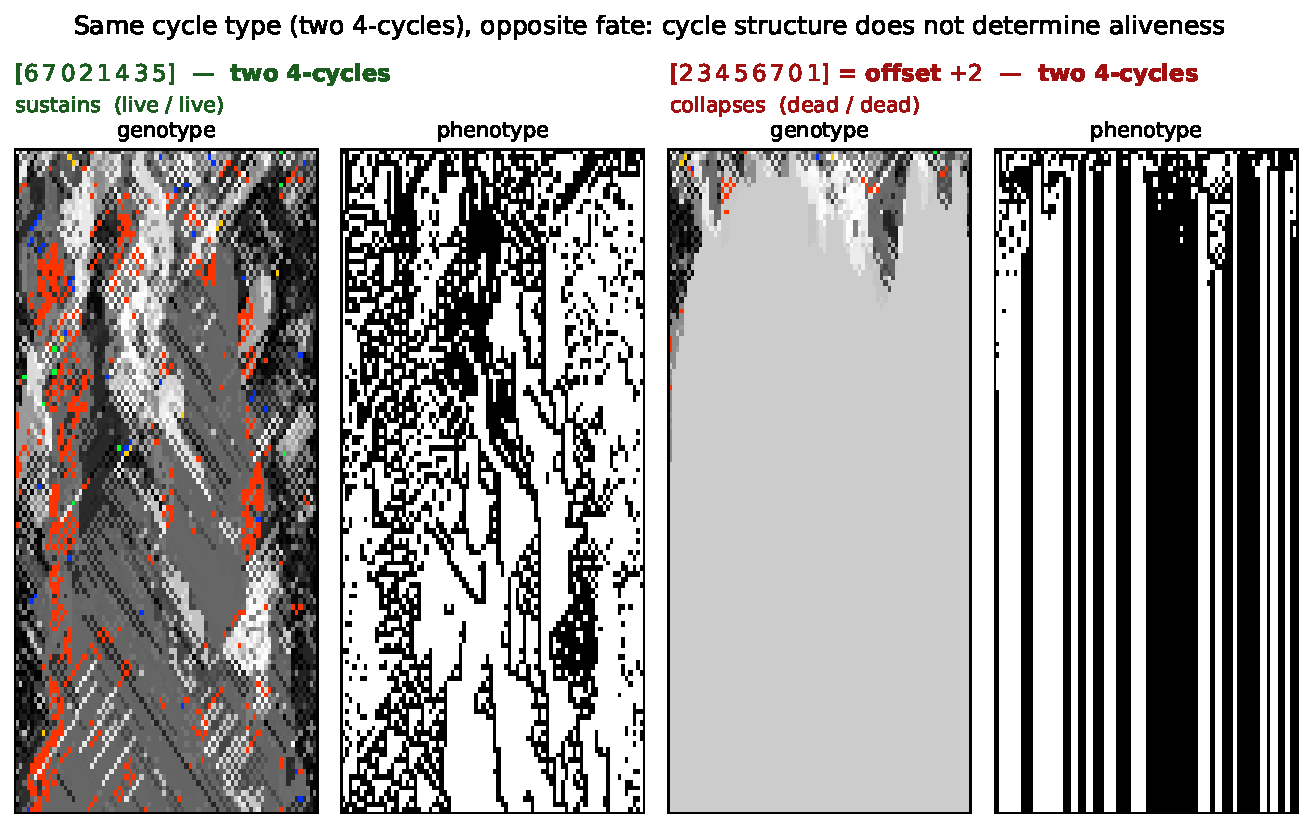
\includegraphics[width=\linewidth]{figures/two4cycle.pdf}
\caption{\textbf{Cycle structure does not determine aliveness.} Two operators of
identical cycle type---both two 4-cycles---with opposite fate. Left,
$[6\,7\,0\,2\,1\,4\,3\,5]$ sustains a live genotype and phenotype; it is the
standard-Wolfram-order form of the historical offset$+2$ operator (its
conjugate). Right, the Wolfram-order rotation offset$+2=[2\,3\,4\,5\,6\,7\,0\,1]$
has the same two-4-cycle structure yet collapses to a dead genotype and a frozen
phenotype. Same cycle type, opposite outcome: the specific permutation, not its
cycle type alone, decides. A full census of the 40320 operators confirms the
two-4-cycle class splits between sustaining and collapsing.}
\label{fig:two4cycle}
\end{figure}

\subsection{Constructive control by temporal schedules}
\label{sec:braiding}

\begin{definition}[fold,label={def:braid}]{Temporal braid}
A \emph{temporal braid} alternates two writings between complete coupled spatial
updates: writing $w_A$ is used at even times and $w_B$ at odd times. More
generally, a periodic \emph{schedule} selects one writing at each time step.
This preserves the intermediate spatial states and neighbour blends; it is not
the algebraic composition $P_{\sigma_A}\circ P_{\sigma_B}$ of two simultaneous
maps.
\end{definition}

\suppfinding{3}{A braid of two collapsing operators can sustain the field}

\begin{figure}[t]
\centering
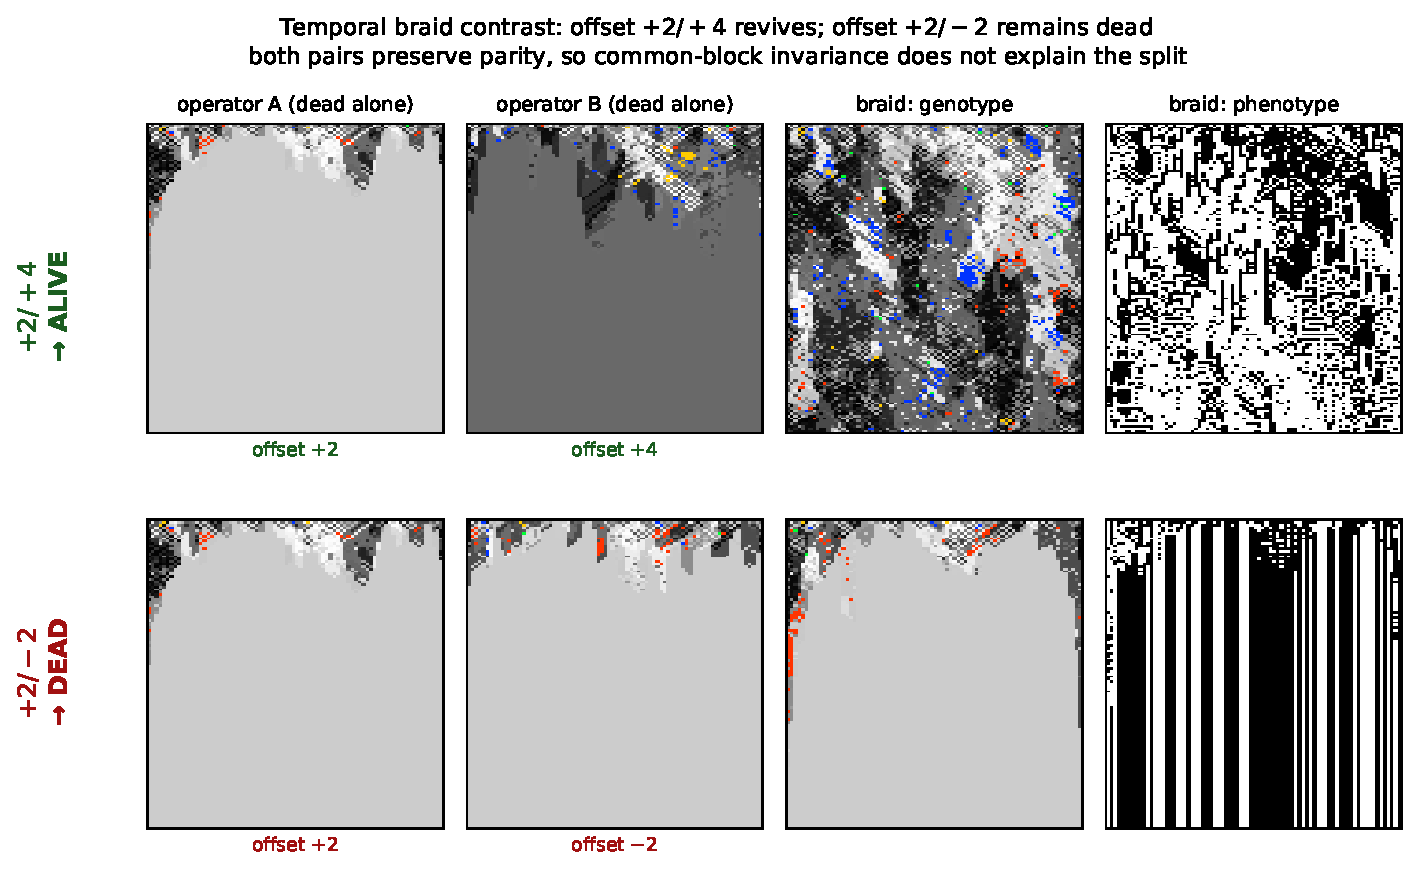
\includegraphics[width=\linewidth]{figures/braid.pdf}
\caption{\textbf{Temporal braiding can sustain aliveness.} Two operators that each collapse
alone are braided by alternating their elementary spatial updates. Top:
offset$+2$ (two
4-cycles) and offset$+4$ (four 2-cycles) are each genotypically dead, yet their
braid is alive (genotype change-rate $0.76$, vs.\ $0$ for either alone). Bottom:
offset$+2$ braided with offset$-2$ stays dead. Both tested pairs preserve parity,
so the contrast is not explained by the existence of that common invariant
partition. The result concerns time-dependent coupled dynamics, not composition
of the simultaneous maps $P_\sigma$.}
\label{fig:braid}
\end{figure}

\suppfinding{4}{The mixing fraction is a reproducible diversity control}

\begin{figure}[t]
\centering
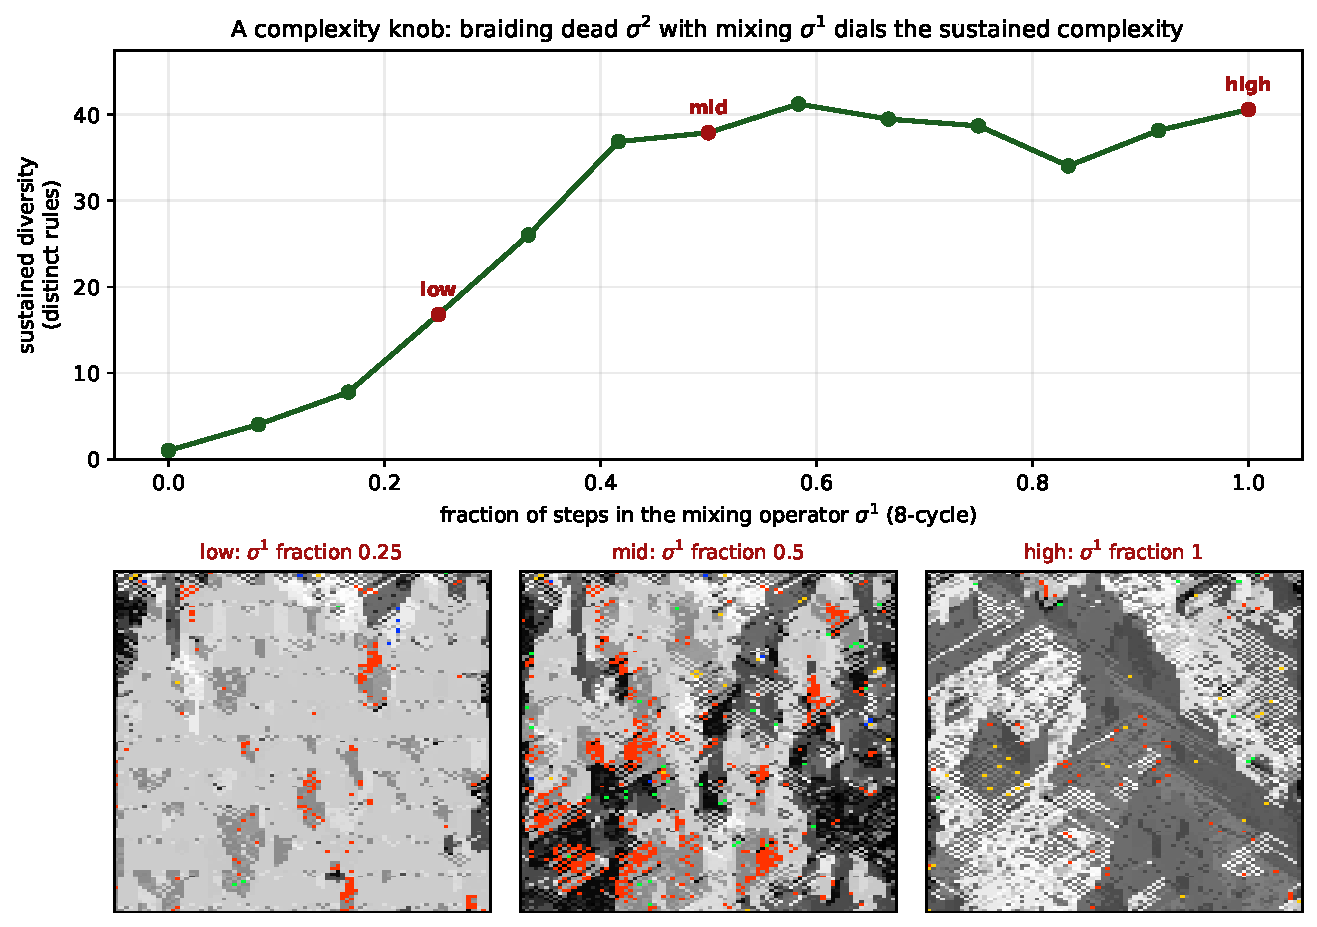
\includegraphics[width=\linewidth]{figures/knob.pdf}
\caption{\textbf{A diversity-control schedule.} Periodic 12-step schedules mix
the sustaining offset-$+1$ operator $\sigma^1$ with the collapsing offset-$+2$
operator $\sigma^2$. Mean late-window distinct-rule diversity (five seeds) rises
from $1.0$ with no $\sigma^1$ steps to a high-diversity plateau once its fraction
reaches roughly $0.4$. The three fields show fractions $0.25$, $0.50$, and $1.0$
at the same representative seed.}
\label{fig:knob}
\end{figure}

\begin{definition}[fold,label={def:interrupter}]{Interrupter}
An \emph{interrupter} is an update between elementary propagator writes that is
not itself a propagator write. The coordinate-wise neighbour blend of
Box~\ref{box:metaca-step} is the interrupter in the ordinary spatial runs; a
hold gate that suppresses a scheduled write is another example. An interrupter
changes the coupled dynamics but does not, by definition, guarantee sustained
diversity.
\end{definition}

\suppfinding{5}{The rotation split occurs with and without neighbour blending}

\begin{proposition}[fold,label={obs:flat}]{Composition parity}
Products alternate between complemented and uncomplemented coordinate permutations.
Each operator of Equation~\eqref{eq:prop} negates every bit
($P_\sig(g)[j] = \lnot\,g[\sig^{-1}(j)]$, a coordinate permutation followed by a
global flip), so under composition the flips cancel in pairs: $P_\sig \circ
P_\tau$ is a \emph{pure} coordinate permutation with no negation left---a
bijection that fixes $2^{c}$ bytes for $c$ cycles but carries none of the forced
$\lambda = 1/2$ structure. An even number of propagators therefore composes to
an uncomplemented coordinate permutation, and an odd number to another member
of the permutation-propagator family.
\end{proposition}

Exploratory searches over products of two and three simultaneous propagators
found no additional structural regime. Temporal braiding is a different
operation: it alternates stochastic elementary writes inside the spatially
coupled dynamics rather than replacing them by one composed map.

Algebraic composition is therefore closed in the sense of
Proposition~\ref{obs:flat}. Temporal scheduling is different: it retains each
intermediate coupled state, which is why the braids of
\secref{sec:braiding} can produce dynamics absent from either held operator. A
second constructive mechanism pairs a propagator with a step of a different
kind.

\section{Limits of the Tested Distance and Complexity Measures}
\label{sec:metrics}

\suppfinding{6}{The tested per-trajectory metrics do not separate the parity classes}

\section{A Parameter-Space Test}
\label{sec:discussion}

The survey (Figure~\ref{fig:eoc}) exposes a sharp behavioural split within a
family of provably fixed-point-bearing operators: only the single 8-cycles
(offset $\pm 1$, $\pm 3$) sustain a high-diversity phase, while offset $\pm 2$ and
$\pm 4$ collapse. A reader is entitled to ask whether that phase sits at a
\emph{critical point}---tuned between an ordered and a disordered phase, as CA
complexity is often supposed to \parencite{langton1990computation}. This is the
first of the two readings distinguished at the outset---an edge of chaos located
in \emph{parameter space}, at some value of a tunable control parameter---and
the finite-size scan below is the test of it, the only place in this paper where
that reading is put to the question. We then ask
whether the sustained diversity is spatially organised into coexisting
dynamical regimes.

\suppfinding{7}{No finite-size evidence of a critical point over the tested range}

The genotype field is also spatially organised. Tinting by activity resolves it
into coexisting low- and high-activity domains whose boundaries trace
fractal-like filamentary walls through spacetime; those walls carry elevated
genotype churn, and at matched activity the two sides hold measurably different
rule populations, so they are not an artefact of the tint that draws them. We
report that structure in Supplement~2, together with a measure of
information transport along those boundaries that we built, validated against
three nulls, and then withdrew when it proved to be an artefact of its own
construction. Neither is a third edge, and nothing in the argument below depends
on them.

\begin{figure}[tb]
\centering
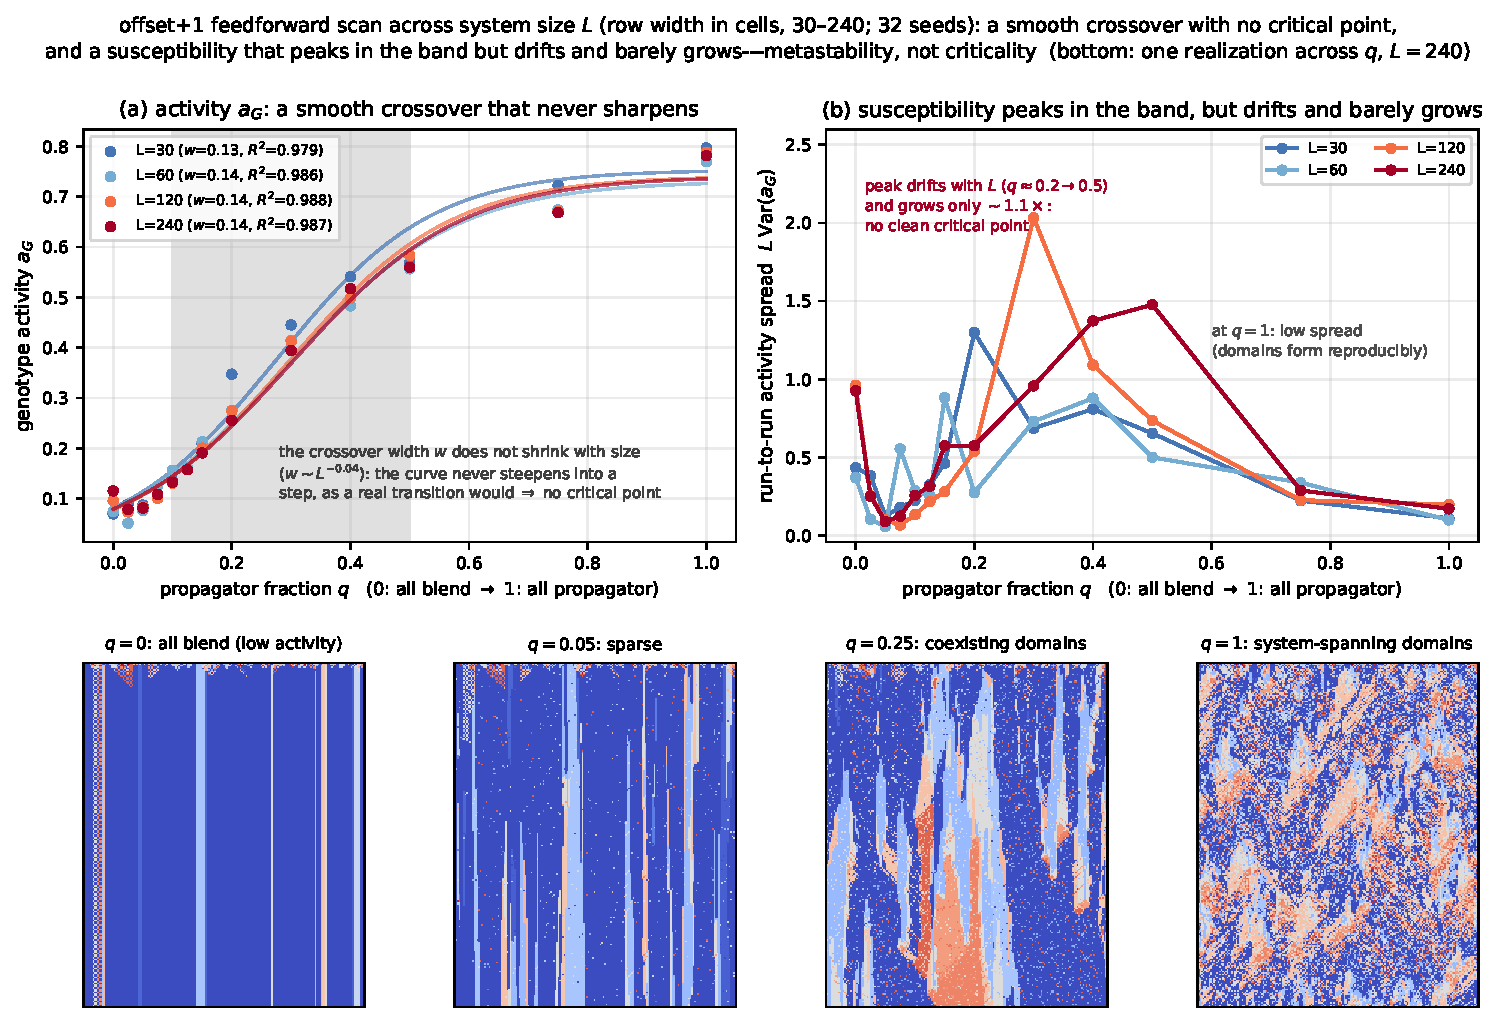
\includegraphics[width=\linewidth]{figures/eoc_phase.pdf}
\caption{\textbf{No finite-size evidence of a critical point over the tested
range.} Offset $+1$ feedforward finite-size scan against the
propagator fraction $q$ ($0$: all blend, $1$: all propagator). $L$ is the
\emph{system size}---the lattice width in cells; the scan spans $L = 30$--$240$
(32 seeds each), because a genuine transition sharpens as $L$ grows while a
crossover does not. \textbf{(a)}~genotype activity $a_G$ with logistic fits
($R^2 > 0.99$); the crossover width does not shrink over these sizes
($w \sim L^{-0.04}$). \textbf{(b)}~the size-scaled run-to-run spread
$L\,\mathrm{Var}(a_G)$ is used as a susceptibility proxy: it peaks inside the
band, but its maximum moves from $q=0.75$ to $0.50$ and then to the sampled
boundary $q=1$ for the two largest sizes; its height grows ${\sim}5.7\times$.
\textbf{(c)}~finite-horizon collapse becomes rarer with size.
\textbf{(d)}~the Binder cumulant has no common crossing. Together these
diagnostics support a broad crossover rather than a confirmed critical point.
Bottom: one paired realisation ($L = 240$, single seed) tinted by isolated-rule
activity at $q=0$, $0.05$, $0.25$, and $0.75$.}
\label{fig:phase}
\end{figure}

\newpage
\part{Beyond the Permutation Core: Feedback and Causal Propagation}
\label{part:feedback}

Part~I's classified object and exhaustive census were the finite permutation
core; its temporal braid was the boundary case, already replacing one held
operator with a schedule. We now retain the same genotype--phenotype lattice
and elementary rule semantics but drop the single-operator restriction. The
objects in Part~II are update architectures: time-dependent schedules,
phenotype-conditioned writes, mutation and holding protocols, and conservative
local transports. Some use writings from the $8^8$ family as components, but a
state-dependent architecture is not itself one fixed writing. Consequently,
the results below neither classify nor measure the $8!$ family as a whole; they
test how causal propagation changes when the genotype update can read the
phenotype.

\section{A Feedback-Coupled Construction}
\label{sec:feedback-construction}

The next construction crosses that boundary by allowing the update to depend
on the live phenotype.

\begin{definition}[fold,label={def:river}]{River}
A \emph{river} is the composed operator obtained by following the collapsing
offset-$+2$ propagator ($\gcd 2$) with a phenotype-reading construction
step---match the local phenotype against four template candidates, first match
wins, and fall back to the all-zero rule when none matches.
\end{definition}

\suppfinding{8}{The river sustains structured phenotype}

\begin{figure}[t]
\centering
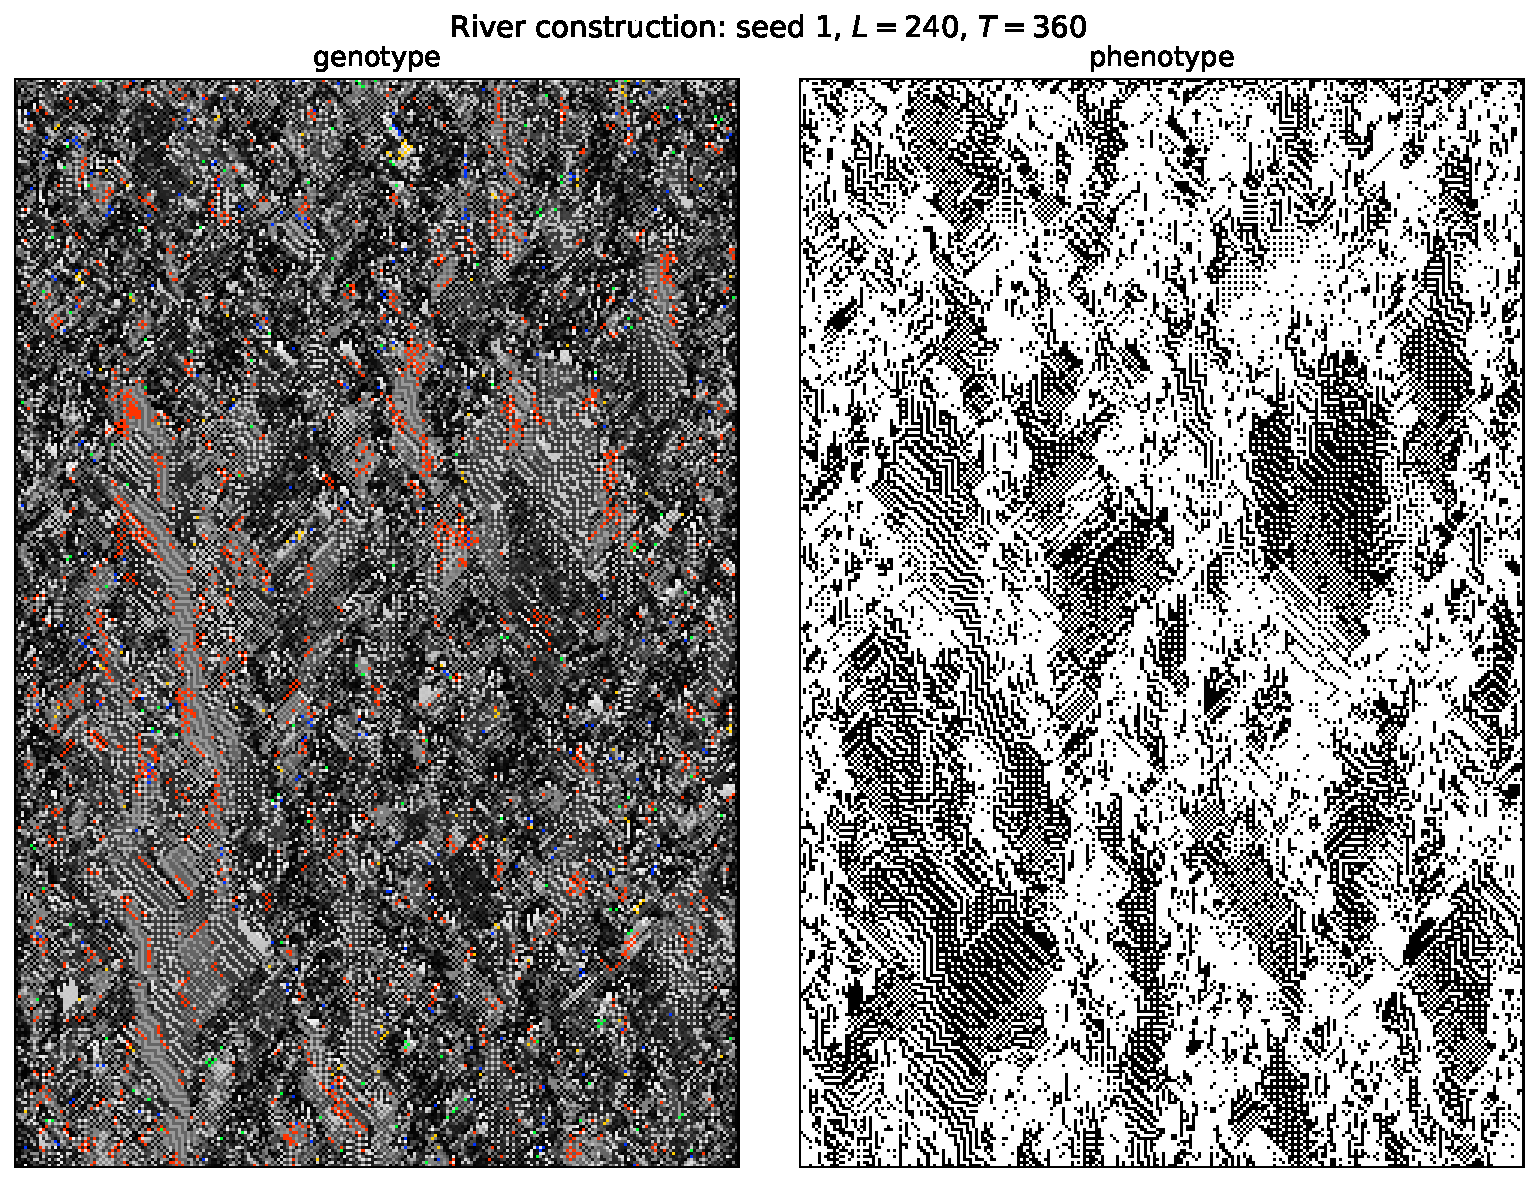
\includegraphics[width=\linewidth]{figures/river.pdf}
\caption{\textbf{A larger river spacetime plate.} One pinned representative
run (seed 1) at $L=240$, $T=360$, with genotype at left and phenotype at
right. The offset-$+2$ propagator is composed with a phenotype-reading,
four-candidate, first-match template construction (fallback: the all-zero
rule). Alternating phenotype domains branch, merge, and reorganise throughout
the run rather than resolving to a homogeneous or short-period field.
Genotype is coloured by rule as in
Figures~\ref{fig:regimes}--\ref{fig:eoc}: greyscale by byte value, with
well-known ECAs highlighted and red denoting Rule~110. Where the bare rotations
collapse or cycle (Figure~\ref{fig:eoc}), this composition sustains structured
phenotype for the length of the observed run.}
\label{fig:river}
\end{figure}

\section{A Causal Measure}
\label{sec:causal}

A causal test also avoids a general problem with observational regions. Any
statistic computed over a region drawn from the field it is computed on invites
circularity, and no null defined only by moving that region can necessarily
detect it. We therefore stop drawing regions: perturb one cell and ask where
the effect arrives.

We run the phenotype-reading construction of
\secref{sec:feedback-construction} to $t^{*}=60$,
fork, flip a single phenotype bit at site $x$, and continue both branches to
$T=120$, recording which cells differ. The fork is exact: the construction draws
one pseudo-random position per cell per step, so re-running from the same seed
gives both branches an identical tape and every divergence is the causal
consequence of the flip. The control is the matched feedback-off variant---same
seed, tape, construction and initial state, with only the live
phenotype-to-genotype edge cut.

\suppfinding{9}{Phenotype-to-genotype feedback roughly doubles causal reach}

\begin{figure}[tb]
\centering
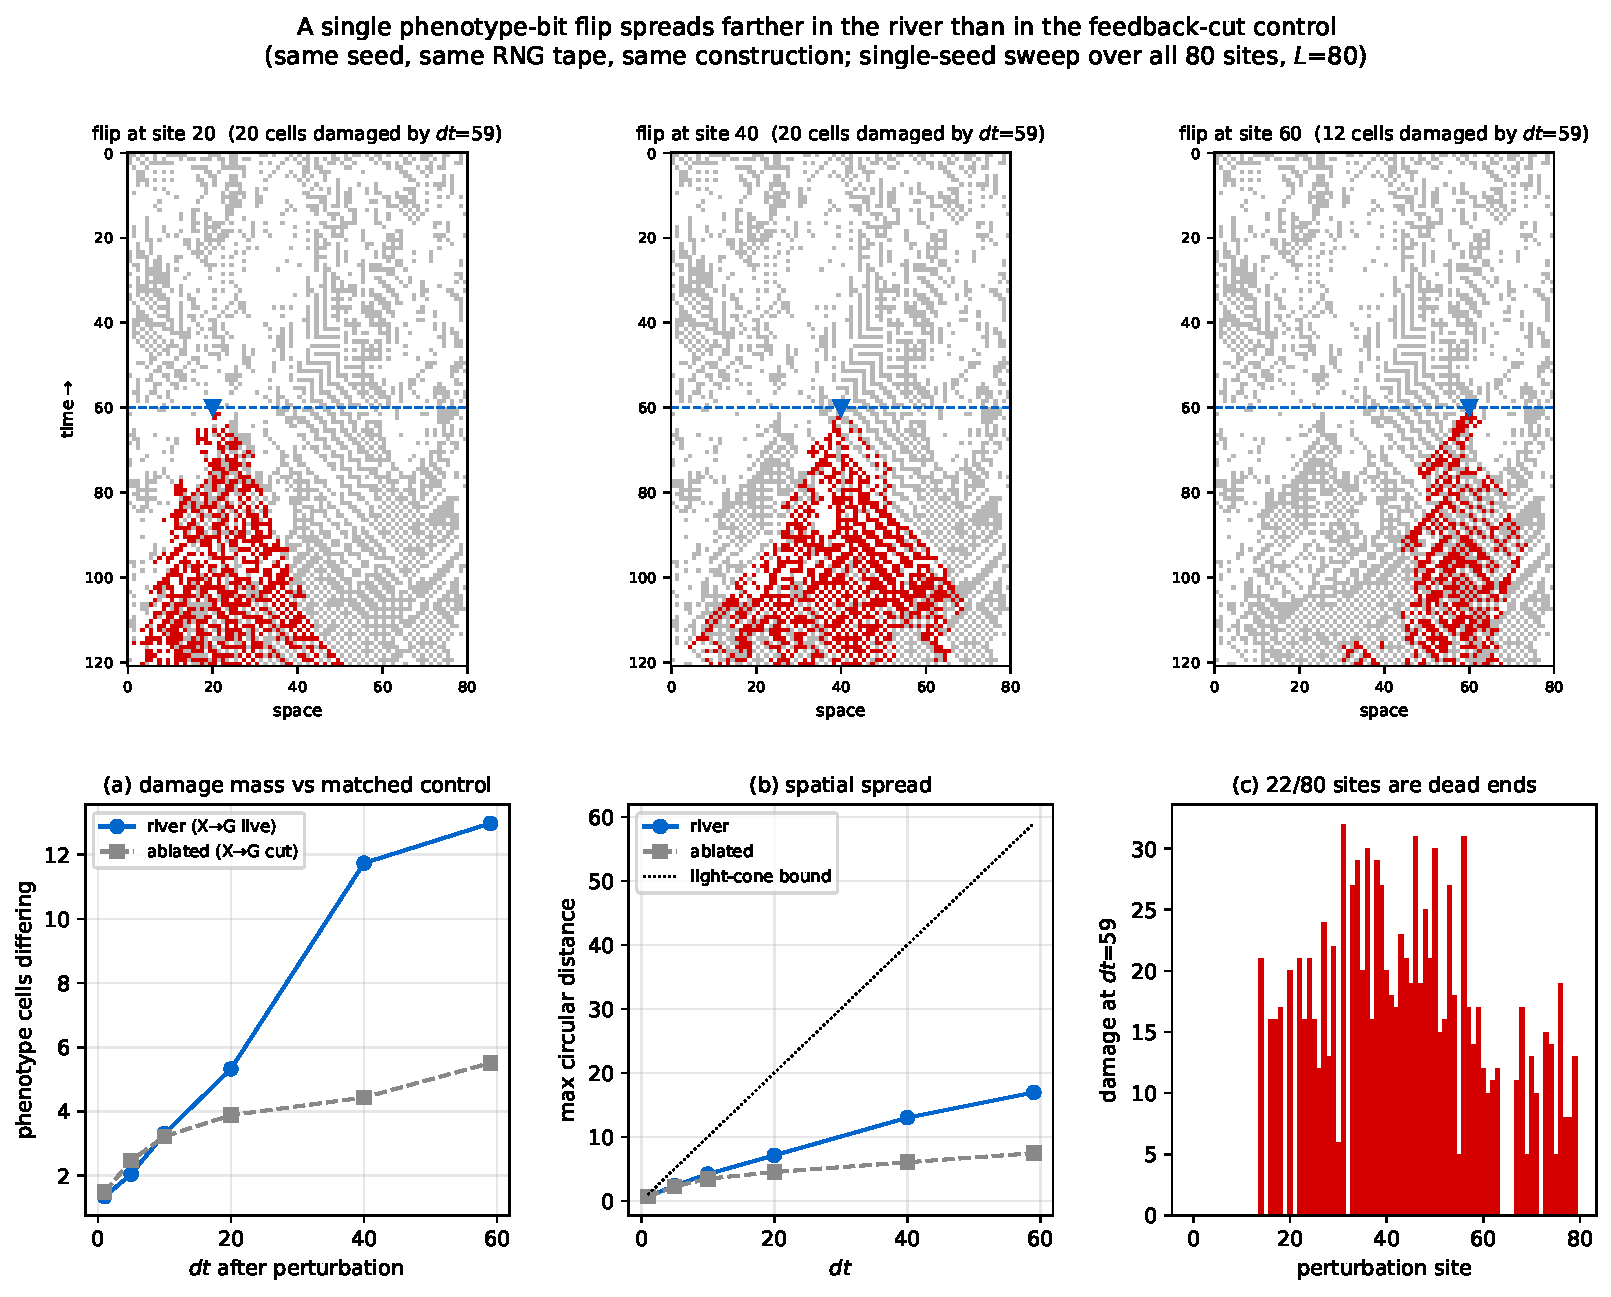
\includegraphics[width=0.94\linewidth]{figures/river_perturbation.pdf}
\caption{\textbf{A causal measure of reach.} A single phenotype bit is flipped
at $t^{*}=60$ (blue marker) and the damage---\emph{phenotype} cells differing
from an otherwise identical run, distance measured as the shorter circular
displacement on the periodic lattice---is tracked. Curves are the single-seed
sweep over all $80$ sites at $L=80$; the six-seed replication is reported in the
text. Top: three light cones at different perturbation
sites. \textbf{(a)}~damaged cells against the matched feedback-off control;
\textbf{(b)}~spatial spread, with the light-cone bound for reference;
\textbf{(c)}~damage by perturbation site, showing a contiguous region of dead
ends. Same seed, same pseudo-random tape, same construction; the two branches
differ only in the live phenotype-to-genotype edge.}
\label{fig:river-perturbation}
\end{figure}

Two readings of that result must be separated. A glider carries a fixed-width
packet at constant velocity; a conductive medium disperses. Tracking the damage
centroid distinguishes them, and the reference values must be measured rather
than assumed---elementary rule $110$, whose gliders support universal
computation, does not give a fixed packet under a random single-site
perturbation, because the perturbation creates and destroys gliders which then
collide.

\suppfinding{10}{Causal reach on a scale calibrated against elementary rules}

\suppfinding{11}{The order parameter is the strength of the phenotype-to-genotype coupling}

\begin{figure}[tb]
\centering
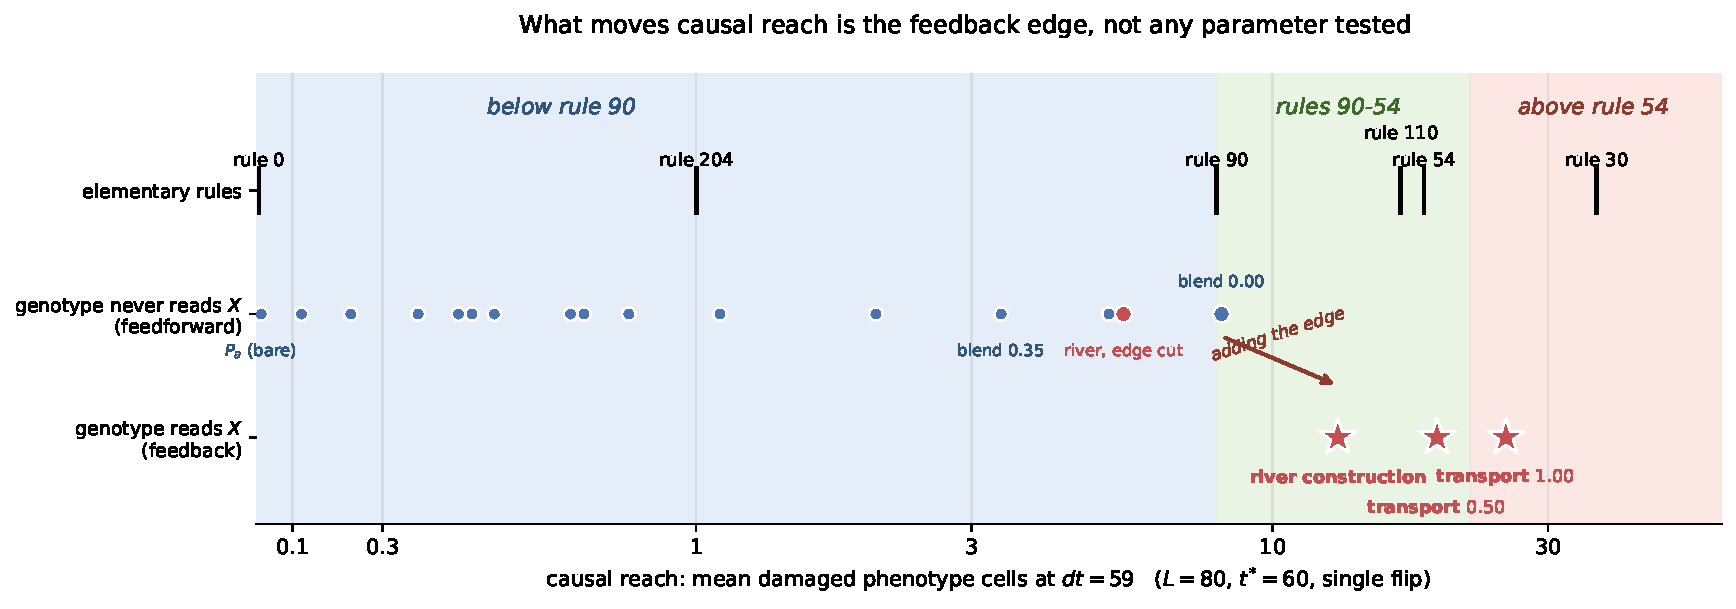
\includegraphics[width=\linewidth]{figures/regime_placement.pdf}
\caption{\textbf{The order parameter is the coupling.} All points share one
protocol ($L=80$, $t^{*}=60$, a single phenotype flip, damaged phenotype cells
at $dt=59$); bands are drawn from the elementary rules, and the calibration
reproduces rules $0$, $204$ and $90$ exactly against
\suppfindingref{10}. \textbf{(a)} Constructions split by
coupling rather than provenance. Nothing whose genotype update is blind to the
phenotype clears the bottom of the complex band---including the ungated
transport controls (squares), which are fully mobile---while everything that
reads it lands inside. The river appears in both rows, at $12.97$ with its edge
and $5.51$ without, so the arrow is one construction moved by adding an edge.
\textbf{(b)} The same coupling as a dial. Gated and ungated transport are both
bijective, both leave the rule histogram invariant, and are matched in mean swap
probability; they differ only in whether the swap reads the local phenotype.
Error bars are standard errors over four seeds and ten sites. The gated curve
crosses rule $90$ between rates $0.10$ and $0.20$ and saturates past rule $54$;
the blind control stays near the frozen identity throughout.}
\label{fig:regime-placement}
\end{figure}


\begin{figure}[tb]
\centering
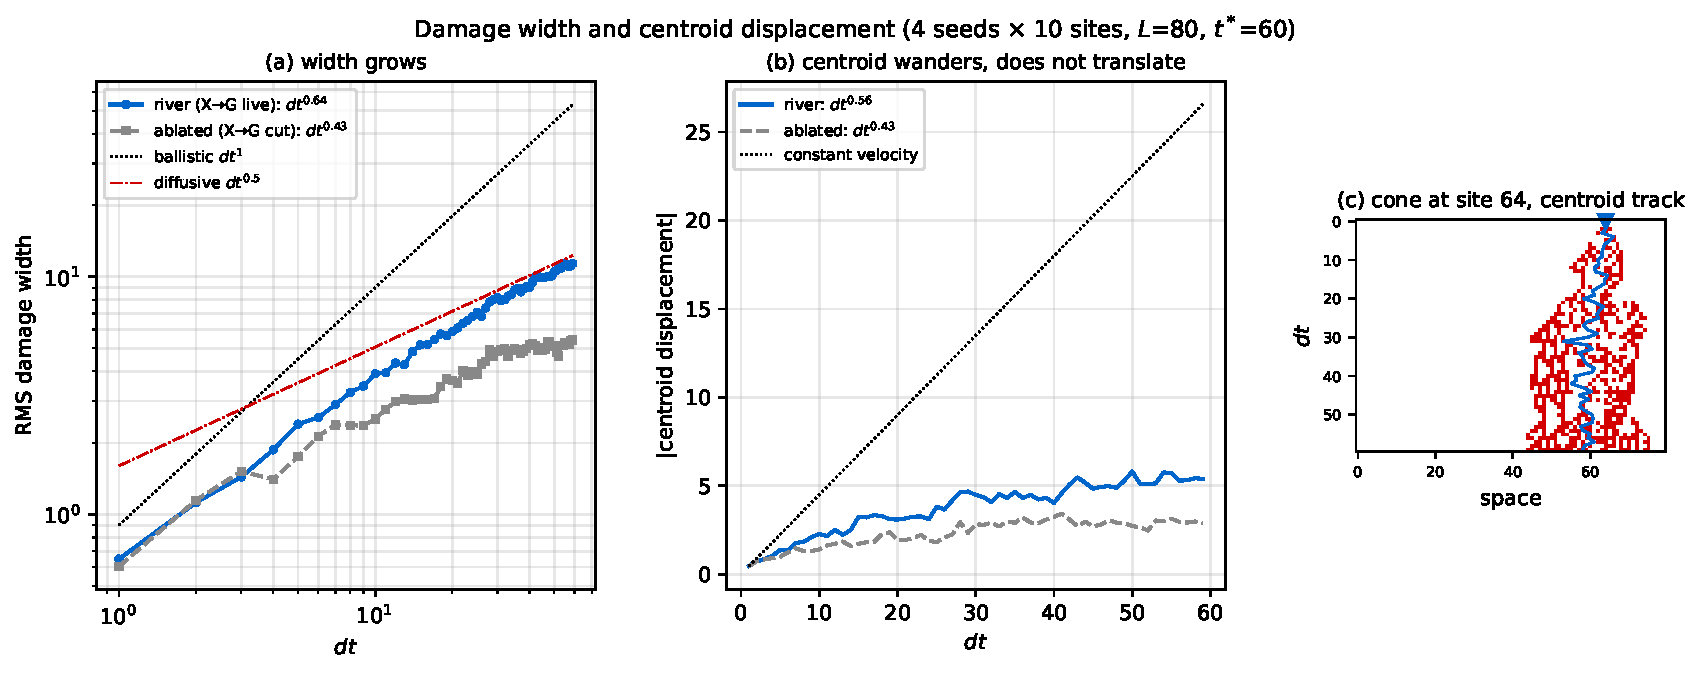
\includegraphics[width=0.94\linewidth]{figures/river_centroid.pdf}
\caption{\textbf{Damage width and centroid displacement.} \textbf{(a)}~damage width against $dt$,
log--log, with ballistic and diffusive references; \textbf{(b)}~centroid
displacement; \textbf{(c)}~a single cone with the centroid track overlaid. The
packet disperses while its centroid stays near the perturbation site. We do not
read this as excluding particle-like transport: under the same protocol rule
$110$, whose gliders support universal computation, gives $dt^{0.68}$ and
$dt^{0.73}$, so a random single-site perturbation does not produce a
fixed-width translating packet even where gliders certainly exist.}
\label{fig:river-centroid}
\end{figure}

\subsection{The coupling as a dial}
\label{sec:gain}

Treating that coupling as present or absent understates it. In both
constructions that read the phenotype it is a quantity, and causal reach is a
graded, monotone function of it.

\suppfinding{12}{Coupling is a dial, not a switch, and reach is monotone along it}

For conservative transport the gain is the phenotype-gated swap rate; reach
crosses rule $90$ between rates $0.10$ and $0.20$ and saturates past $0.75$. For
the river it is the \emph{currency} of the phenotype bits the genotype reads:
each cell at each step reads the live phenotype with probability $\gamma$ and a
frozen reference otherwise, so $\gamma$ is the fraction of the genotype's view
that is causally current. Because the frozen field is itself a real phenotype,
marginals and spatial structure are matched at every $\gamma$ and only causal
currency varies; because $\gamma = 1$ reproduces the live river exactly, the
dial is anchored against a measurement made independently of it.

Two consequences bear on the reading of \secref{sec:causal}. First, the
$\gamma = 0$ endpoint is $1.28$, not the $5.51$ of the ablated control: that
control freezes the phenotype the genotype reads but still presents a field
which, in the perturbed branch, contains the flip. It cuts the \emph{currency}
of the read, not the read. The doubling reported for it is therefore the smaller
part of a coupling effect that spans an order of magnitude.

Second, the two dials have opposite curvature (Figure~\ref{fig:gain-curves}).
Transport is concave and buys most of its reach early; the river is convex, with
$45$\% of its span in the last eighth of $\gamma$, so one stale read in eight
costs $40$\% of the reach. Monotonicity in the coupling is thus common to both
constructions while its shape is not, and we would not generalise the shape from
two cases.

\begin{figure}[tb]
\centering
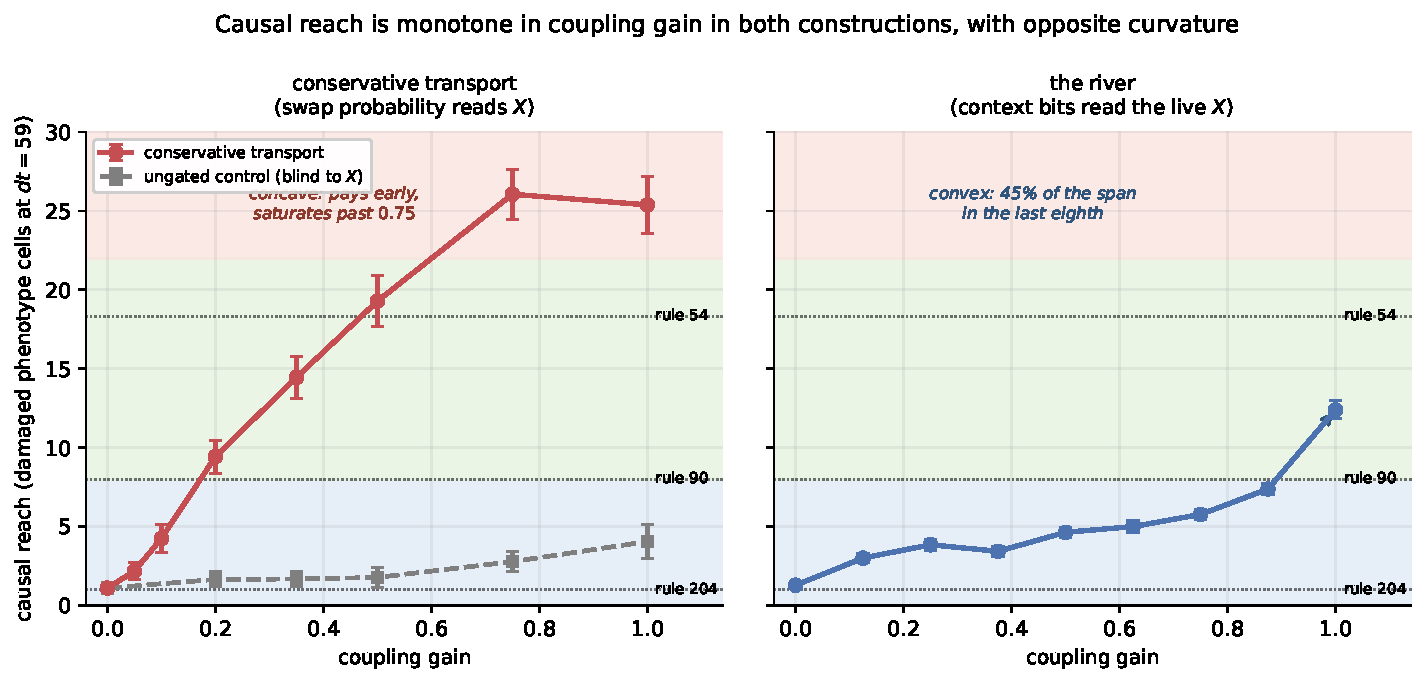
\includegraphics[width=\linewidth]{figures/gain_curves.pdf}
\caption{\textbf{Two couplings, dialled.} Both panels vary the gain of the
phenotype-to-genotype loop and nothing else, under the protocol of
\suppfindingref{10}; bands are the elementary-rule regimes of
Figure~\ref{fig:regime-placement}. \textbf{Left:} conservative transport, whose
swap probability is gated on the local phenotype interface, against an ungated
control at matched mean swap probability---both bijective, both leaving the rule
histogram invariant, differing only in whether the swap reads the phenotype. The
blind control never leaves the ordered band. \textbf{Right:} the river, where
the gain is the fraction of the genotype's phenotype read that is causally
current. Error bars are standard errors over three seeds and eighty sites.
Reach is monotone in gain in both, with opposite curvature: transport saturates
past $0.75$, while the river gains $45$\% of its span in the last eighth.}
\label{fig:gain-curves}
\end{figure}

\subsection{Diversity and conservative transport}
\label{sec:diversity-axis}

Langton's $\lambda$ is silent on this family: the classification puts
\emph{every} fixed rule of \emph{every} operator at $\lambda = 1/2$, so it
cannot distinguish an operator whose field stays diverse from one that
collapses. It cannot be rescued by computing it on the realized dynamics
either. Across the nine configurations of
Figure~\ref{fig:diversity-spread} the empirical neighbourhood distribution is
close to uniform---normalised visitation entropy $0.946$ to $0.999$, all eight
neighbourhoods visited in every run---so $\lambda$ read off the realized
transitions with uniform weight ($0.42$ to $0.52$) and the same quantity
weighted by visitation ($0.40$ to $0.51$) differ by $0.035$ on average, and both
sit near $1/2$ wherever the nominal value does. Nor is the silence peculiar to
this family: of the elementary rules calibrating the scale above, rules $30$,
$54$, $90$, $150$, $204$ and $232$ all have $\lambda = 1/2$ exactly, spanning
frozen, ordered, complex and chaotic. What the balance theorem contributes is
not a new failure of $\lambda$ but an exact and provable instance of a known
one. The sustained distinct-rule count can, and the causal measure above
lets us ask the stronger question: does causal reach depend on diversity
itself, or on the mechanism used to sustain it?

Our initial survey varied sustained diversity by seven mechanisms that share little: the bare
operator family; braided writings; the fork time after seeding the genotype with
a randomised \emph{full} rule population; a continuous blend strength; random
rule mutation; asynchronous refuges that hold a cell's rule exactly with some
probability; and spatially phase-shifted braid niches. A limiting case anchors
the top of the range: a genotype held fixed at the full population has maximal
diversity and no rewriting at all. The coordinate throughout is diversity
\emph{sustained through the response window}, not diversity at the instant of
the fork---a field seeded with all $256$ rules holds them for one step and
collapses during the very window the damage is measured in.

\suppfinding{13}{Sustained diversity does not determine causal reach; conservative transport breaks the apparent interior optimum}

\begin{figure}[tb]
\centering
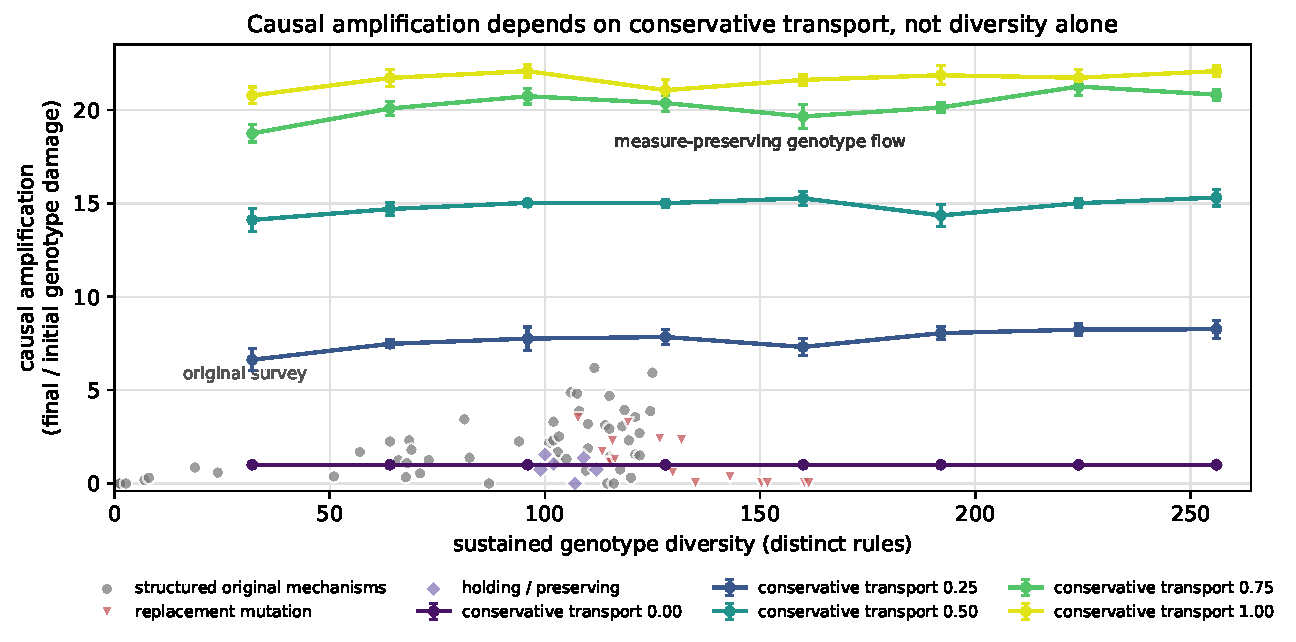
\includegraphics[width=\linewidth]{figures/diversity_axis.pdf}
\caption{\textbf{Causal reach against sustained genotype diversity.}
The original $76$ configurations appear in the lower part of the panel, grouped
as structured mechanisms, replacement mutation, and holding or preservation.
Their apparent descending limb above $135$ rules is mechanism-confounded.
Coloured curves show the conservative-flow control: prescribed balanced
measures of $32$--$256$ distinct rules, transported only by local bijective
exchanges at five rates. Points are means over six seeds after averaging eight
perturbation sites within each seed; bars are standard errors across seeds.
Causal amplification is final divided by initial genotype damage, leaving the
original one-site intervention unchanged and normalising the conservative
two-site exchange by two. At every non-zero transport rate, reach is sustained
across the entire diversity range. The vertical separation by transport and
near-flat curves within rate show that transport mechanism, not diversity
alone, governs propagation.}
\label{fig:diversity-axis}
\end{figure}

\begin{figure}[p]
\centering
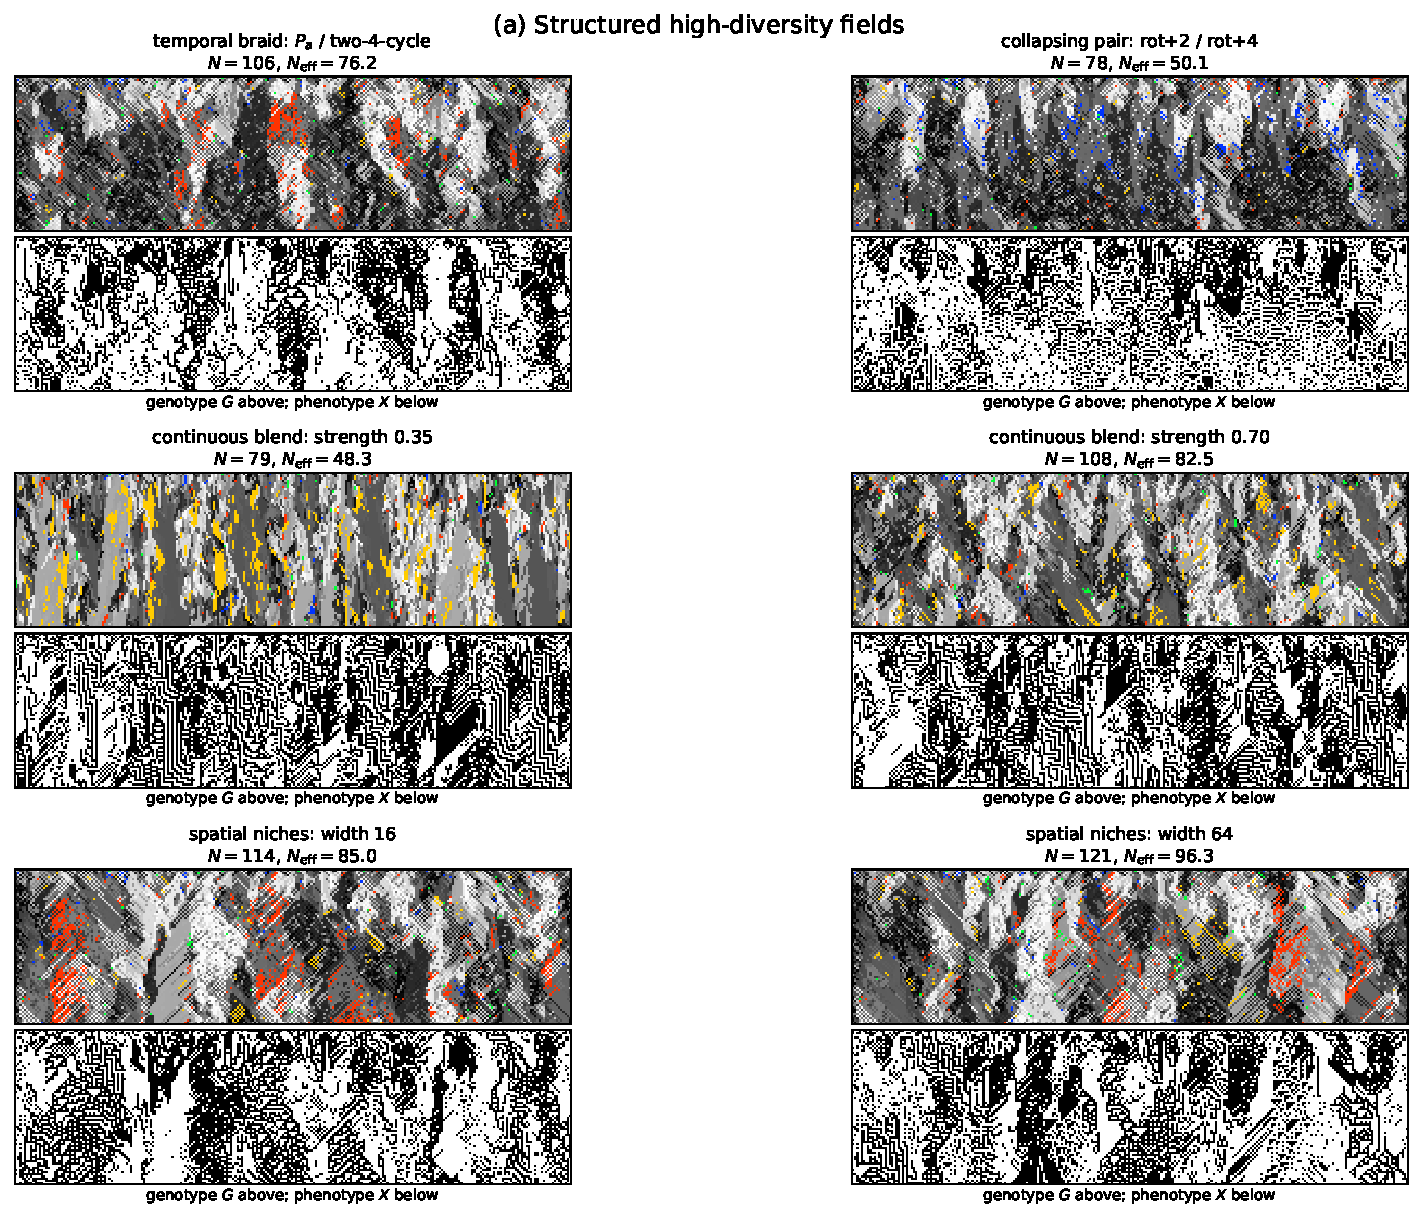
\includegraphics[width=\linewidth]{figures/diversity_spread_a.pdf}
\caption{\textbf{(a)~Structured high-diversity fields.} Six examples from four
mechanism families: temporal alternation; alternation of two operators that
\emph{collapse} when run alone; continuous blending at two strengths; and
spatial niches at two widths. Each tile stacks genotype over phenotype and
reports both distinct-rule and Shannon-effective diversity at $T=70$;
full-population seed $0$, $L=256$. The fields sustain $78$--$121$ rules and
carry coherent diagonal structure at a range of scales. These examples
motivated the candidate diversity coordinate, but the conservative-flow control
in Figure~\ref{fig:diversity-axis} shows that diversity itself does not account
for their propagation.
Continued in~(b).}
\label{fig:diversity-spread}
\end{figure}

\begin{figure}[p]
\ContinuedFloat
\centering
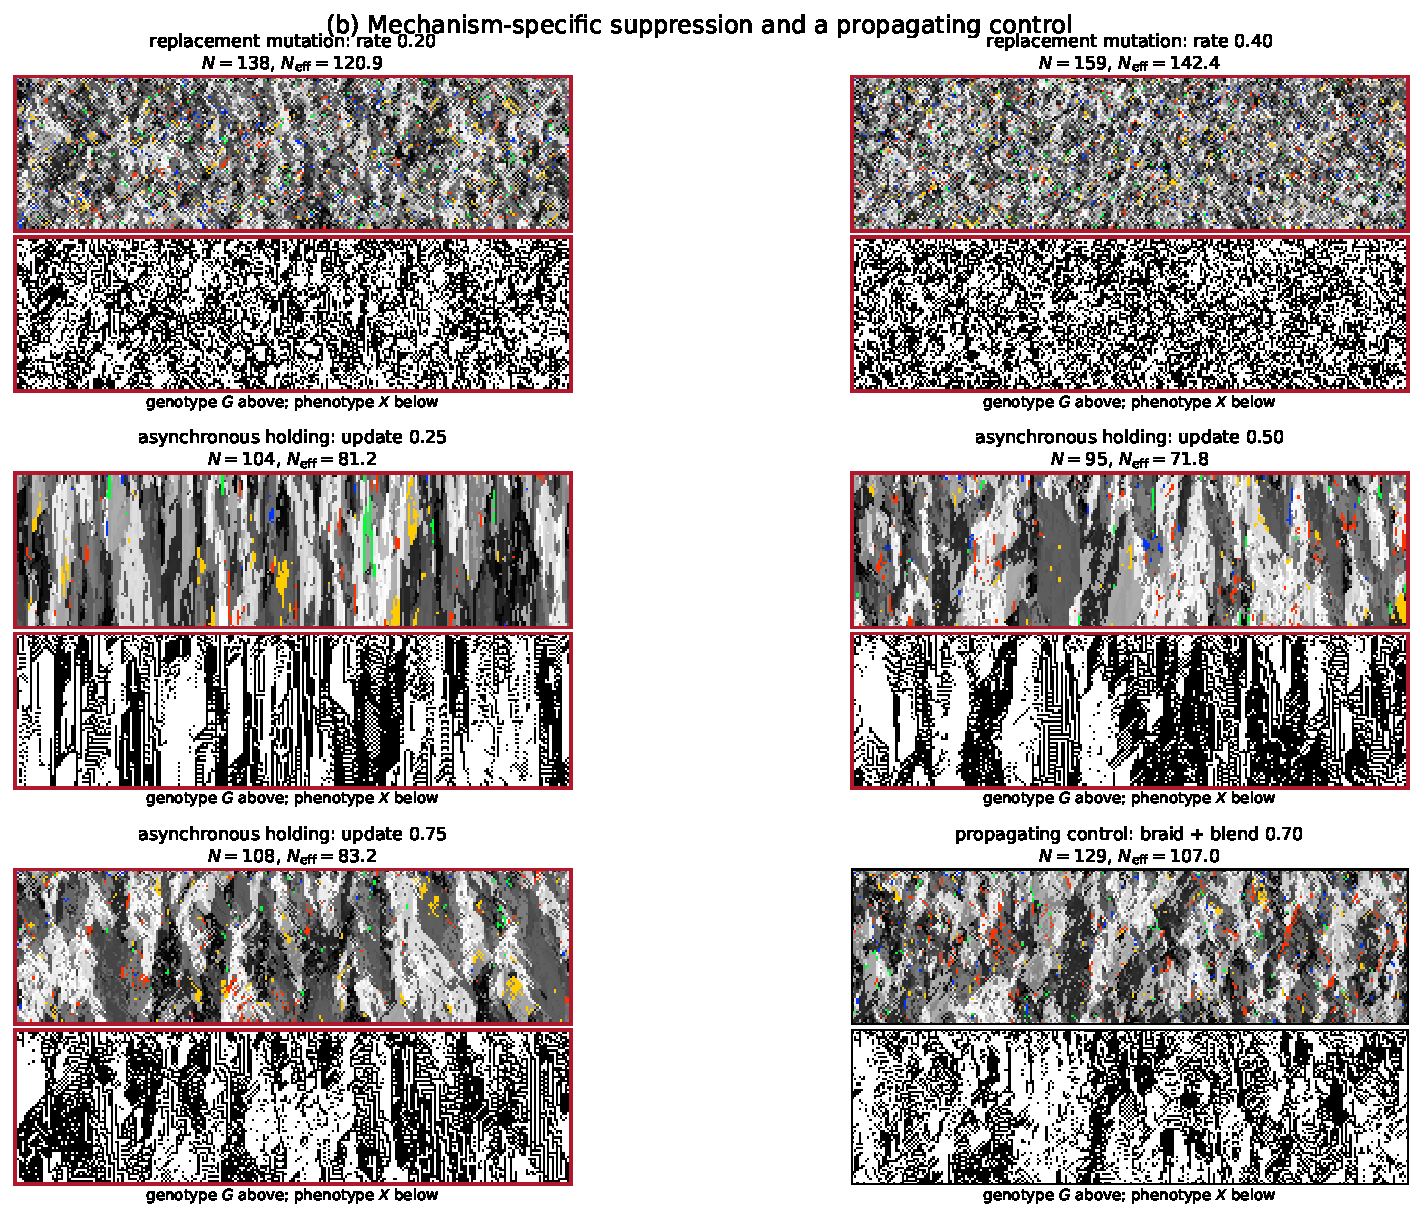
\includegraphics[width=\linewidth]{figures/diversity_spread_b.pdf}
\caption{\textbf{(b)~Two mechanism-specific suppressions.} Continued from~(a);
suppressed configurations are outlined in red. Replacement mutation at rates
$0.20$ and $0.40$ turns the genotype into progressively finer, unstructured
speckle. Asynchronous holding at update fractions $0.25$, $0.50$, and $0.75$
instead produces vertical persistence whose strength changes continuously with
the dial. The unoutlined braid-plus-blend control at bottom right propagates
($3.88$ cells) and recovers the diagonal texture of~(a). The expanded
population makes the distinction visible as a family resemblance rather than a
single selected contrast: these are genuine failure modes of their respective
mechanisms, not evidence for suppression by high diversity.}
\end{figure}

Two cautions bound this result. First, the conservative intervention is a local
transposition, rather than the one-bit, one-site intervention of the original
survey. Normalising by initial damage puts their amplification on a common
scale, but the conservative curves are a falsification control, not a claim
that their absolute heights rank all mechanisms. Second, phenotype-gated
bijective exchange is one deliberately constructed transport law, tested at one
lattice width and one response horizon. It establishes existence: fields can
remain mobile and propagate damage at effective diversities well above $135$
without mutation. It does not establish that transport rate is a universal
order parameter.

The defensible conclusion is narrower and cleaner. Distinct-rule diversity
describes population persistence in the Part~I operator experiments, but it
does not govern causal reach across the Part~II architectures. The latter
depends on how rewriting or transport is organised. Identifying a coordinate
that captures that organisation across mechanisms is work for another paper;
the classification of \secref{sec:classification} guarantees only that
$\lambda$ cannot discriminate among fixed points in the permutation core.

What this scale does and does not license needs saying plainly. It separates
systems that propagate a perturbation from those that do not, and that
separation is sharp: frozen rules return exactly zero. It is \emph{not} a
regime coordinate. Wolfram class~III rules bracket the range at both ends---rule
$90$ at $8.00$ and rule $30$ at $37.50$---with the class~IV rules $54$ and
$110$ between them, so a position on this axis does not by itself classify a
system as ordered, complex or chaotic, and we make no such classification. What
we claim is narrower and causal: the live phenotype-to-genotype edge roughly
doubles how far a single-cell perturbation reaches, on a measure that involves
no region-drawing and therefore cannot fail in the way the withdrawn measure of
the Supplement~2 analysis failed. It concerns the phenotype-coupled construction, not the bare operators;
no comparable measurement of the family is attempted here.

\subsection{What the coupling supplies}

One measurement bounds how the convexity of \secref{sec:gain} should be read.
Asking, per cell and step, whether the live phenotype context selects a
\emph{different} rule than a frozen context would: it does in $73.1$\% of
cell-steps (and in $76.8$\% against no context), over four seeds at $L=80$ for
$120$ steps. The construction's first-match runs over four candidates, so an
uninformative re-selection would differ in about $75$\% of cases: at $73.1$\% a
frozen context carries almost no information about the live answer. The read is
determinative rather than a tiebreak, which is what a convex gain curve should
lead one to expect, and it means there is no common case that a
phenotype-blind rule could encode in its place. We draw no stronger conclusion
from this than that: whether \emph{any} blind construction could match the
river is a question about a search we have not run, and
\suppfindingref{9} reports only that sixteen hand-chosen ones do not.

\section{Limits}
\label{sec:limits}

The Part~I theorems are exact for the Boolean permutation core; its dynamical
claims are narrower and empirical. The census uses three seeds per operator,
the rotation survey two, and the finite-size scan $32$ per parameter cell, all
under the stated radius-one spatial protocol. These finite-run results do not
turn fixed-point balance into a claim about attraction. The substrate itself is
not new (\secref{sec:object}), and $\lambda$ is one heuristic among several
\parencite{wuensche1999classifying}; what is exact is only that the fixed-point
structure of Equation~\eqref{eq:prop} forces every fixed rule in the core to
have $\lambda=1/2$.

Part~II has different limits because it has a different object. Its central
causal comparison concerns one feedback-coupled construction rather than
either writing family, one lattice width, and six seeds. The descriptive
exponents are fitted over a range where damage width reaches only a tenth of
the lattice, so finite-size effects are not excluded. The architecture survey
and conservative-transport control compare mechanisms rather than exhaustively
sampling $8^8$ writings, and their fixed sample sizes are stated with each
result. They identify feedback and transport as controls in the tested
constructions, not as universal order parameters. Illustrative diagrams use
pinned representative seeds. All reported computations are reproducible from
the accompanying package.

Supplement~2 carries the separate spatial-domain analysis and the information
measure withdrawn after its mask and measure proved circular. Its claims and
failures do not enter either Part~I's classification or Part~II's causal
comparison.

\section{Conclusion}
\label{sec:conclusion}

The paper has studied two related objects, and its conclusions must keep them
separate. Part~I concerns the finite permutation core. Its static results are
exact: a permutation-propagator possesses fixed rules exactly when all cycles
are even; an all-even permutation with $k$ cycles has $2^k$ fixed rules; and
every such rule is balanced, with $\lambda=1/2$. Its dynamical results are
finite-run observations over that core. The exhaustive census shows that all
odd-cycle operators remain genotype-alive under the stated protocol while
every all-even cycle type contains both sustaining and collapsing members. The
rotation survey and finite-size scan sharpen the distinction: fixed-point
existence does not determine attraction, and the tested propagator-fraction
scan gives a broad crossover rather than evidence of a critical point.

Part~II retains the two-layer lattice but changes the object from an individual
writing to an update architecture. The river construction composes a
permutation-propagator with a phenotype-reading step; the wider comparison adds
temporal schedules, mutation, holding, niches, and conservative local
transport. These are not a census of the $8^8$ writings, and the results do not
retroactively characterise the $8!$ core. They establish a narrower causal
claim. Against a matched feedback-off control, phenotype-to-genotype feedback
roughly doubles the reach of a single-cell perturbation. When the strength of
that feedback is varied, reach changes monotonically, while a control matched
in rule mobility but blind to the phenotype remains in the low-reach band.
Conservative transport further shows that sustained genotype diversity is not
itself the governing coordinate: high diversity can coexist with propagation,
and transport changes reach far more than diversity does.

The connection between the parts is therefore motivational rather than
deductive. Part~I proves that the classical $\lambda$ coordinate cannot
discriminate among fixed points in the permutation core and finds no critical
point in the tested parameter scan. Part~II asks what a causal measurement can
reveal once the architecture itself is allowed to change. Its answer is
feedback coupling for the constructions tested here, not a theorem about all
permutations or all writings. Supplement~2 records the separate spatial-domain
analysis and the withdrawn boundary statistic; neither is a premise of this
two-part argument.

\paragraph{Data and code availability.} Every numerical result in this paper is
regenerated from source rather than deposited: the generators are seeded, so a
single documented command rebuilds the fields underlying the tables, figures,
and reported summary statistics from an empty data directory, and the analysis
scripts consume no input that command does not produce. The code and those
commands are publicly available at
\texttt{https://github.com/tothedarktowercame/mmca-clj} (commit
\texttt{e3e7bc59a02a229ef87bc7b7f296be0f5dc4b0c6})---a standalone,
dependency-light Clojure port of the MetaCA dynamics whose \texttt{README} gives
the complete reproduction command and commands for individual figure groups.
The classification and balance theorems are
formally verified in Lean~4 with Mathlib at
\texttt{https://github.com/tothedarktowercame/mathlib4}, branch \texttt{darktower}
(commit \texttt{bc34d8cec27216aae1d3cd511a9950ab1bce3575}), in
\texttt{DarkTower/Patterns/Propagator.lean}: the cycle-parity criterion as
\texttt{hasAlternatingColouring\_iff\_cycleType\_even} and the $\lambda = 1/2$
balance as \texttt{alternatingColouring\_true\_card\_eq\_four}. The same file
also contains executable regressions for both hand calculations, including the
displayed-position versus numerical-neighbourhood indexing contrast.

\paragraph{Generative-AI disclosure.} Anthropic Claude (Opus~4.8, Opus~5, and
Fable~5) and OpenAI Codex (version 5.6-sol) coding agents
\parencite{anthropic_claude,anthropic_fable,openai_codex} assisted in an
iterative, human-supervised workflow with manuscript editing, software
implementation, test construction, and adversarial checks. Exchanges with
Claude Fable~5 contributed to the initial identification of the operator family
reported here. The author reviewed the resulting prose and code, reran the
reported computations and formal checks, and accepts full responsibility for
the manuscript. Product information was accessed in July~2026; per-source
access dates are given in the bibliography.

\printbibliography
\end{document}
